\documentclass[11pt,a4paper,reqno]{amsart}

\usepackage[T1]{fontenc}
\usepackage{lmodern}
\usepackage[utf8]{inputenc}
\usepackage{amsmath,amssymb,amsthm,mathtools}
\usepackage{booktabs,array,multirow}
\usepackage{graphicx}
\usepackage[margin=1.1in]{geometry}
\usepackage{microtype}
\emergencystretch=1.5em
\usepackage{enumitem}
\usepackage{xcolor}
\definecolor{linkblue}{RGB}{0,51,102}
\definecolor{citeburgundy}{RGB}{128,0,32}
\usepackage[colorlinks=true,linkcolor=linkblue,citecolor=citeburgundy,urlcolor=linkblue]{hyperref}

\newtheorem{theorem}{Theorem}[section]
\newtheorem{proposition}[theorem]{Proposition}
\newtheorem{lemma}[theorem]{Lemma}
\newtheorem{corollary}[theorem]{Corollary}
\theoremstyle{definition}
\newtheorem{definition}[theorem]{Definition}
\theoremstyle{remark}
\newtheorem{remark}[theorem]{Remark}

\numberwithin{equation}{section}

\newcommand{\R}{\mathbb{R}}
\newcommand{\C}{\mathbb{C}}
\newcommand{\Z}{\mathbb{Z}}
\newcommand{\N}{\mathbb{N}}
\newcommand{\Q}{\mathbb{Q}}
\newcommand{\dd}{\mathrm{d}}
\newcommand{\ii}{\mathrm{i}}
\newcommand{\ee}{\mathrm{e}}
\DeclareMathOperator{\Reop}{Re}
\DeclareMathOperator{\Imop}{Im}

\title[P\'olya--Schur Multipliers and $\Lambda_{\mathrm{DH}}$ Bounds]{Stieltjes Regimes of P\'olya--Schur Multipliers and Strict de~Bruijn--Newman Bounds for the Davenport--Heilbronn Function}

\author{Thijs Missiaen}
\address{Independent Researcher, Belgium (ORCID: \href{https://orcid.org/0009-0007-3678-0810}{0009-0007-3678-0810})}
\email{thijs.missiaen@gmail.com}
\date{November 2026}

\subjclass[2020]{Primary 11M41, 11M26; Secondary 30D15, 26C10, 65G20}
\keywords{de~Bruijn--Newman constant, Davenport--Heilbronn function, P\'olya--Schur multipliers, Laguerre--P\'olya class, Gauss--Weierstrass heat evolution, Bohr--Kronecker theorem, interval ball arithmetic}

\begin{document}

\begin{abstract}
We classify the action of real entire P\'olya--Schur multipliers $G(-\partial_z^2)$ on the completed Davenport--Heilbronn function $\Xi_{\mathrm{DH}}(z)$ and establish strict unconditional upper and lower bounds for its de~Bruijn--Newman constant $\Lambda_{\mathrm{DH}}$. Expressing the asymptotic multiplier shift through the Stieltjes logarithmic derivative $S_G(u) = \frac{\dd}{\dd u}\log G(u^2)$, we partition Laguerre--P\'olya multipliers into three regimes governed by the Bohr--Kronecker supremum $\sigma^*$ of $\mathcal{D}_{\mathrm{DH}}(s)$, construct lacunary canonical products showing that upper order $\rho(G) \in (1/2,1)$ fails without root-gap regularity, and certify in interval ball arithmetic that P\'olya's hyperbolic sinc multiplier strictly separates global real-rootedness from the infinite-height Kronecker threshold. Combining a shifted Gauss--Weierstrass contour analysis and equilateral-hyperbola contraction with interval-certified off-real heat-flow witnesses and Platt--Trudgian's bound $\Lambda_\zeta \le 1/5$, we prove unconditionally that $\Lambda_\zeta \le 1/5 < 1153/5000 < \Lambda_{\mathrm{DH}} < 2(\sigma^* - 1/2)^2$.
\end{abstract}

\maketitle

\section{Introduction}
\label{sec:intro}

Let $\chi_5$ denote the odd primitive Dirichlet character modulo~$5$ given by $\chi_5(1)=1$, $\chi_5(2)=\ii$, $\chi_5(3)=-\ii$, $\chi_5(4)=-1$, and $\chi_5(5)=0$, and consider the self-dual Dirichlet combination introduced by Davenport and Heilbronn \cite{davenport1936} (see Titchmarsh \cite[\S 10.25]{titchmarsh1986}):
\begin{equation}
  \kappa := \frac{\sqrt{10 - 2\sqrt{5}} - 2}{\sqrt{5} - 1},
  \qquad
  \mathcal{D}_{\mathrm{DH}}(s) := \frac{1 - \ii\kappa}{2}\,L(s,\chi_5) + \frac{1 + \ii\kappa}{2}\,L(s,\overline{\chi_5})
  = \sum_{n=1}^{\infty} a_{\mathrm{DH}}(n)\,n^{-s}.
  \label{eq:dh-series}
\end{equation}
In the canonical normalization of Riemann \cite{riemann1859}, P\'olya \cite{polya1926,polya1927}, de~Bruijn \cite{debruijn1950}, and Newman \cite{newman1976}, the completed entire function and its theta-kernel cosine representation take the form
\begin{equation}
  \begin{aligned}
    \xi_{\mathrm{DH}}(s) &:= \left(\frac{5}{\pi}\right)^{(s+1)/2}\Gamma\!\left(\frac{s+1}{2}\right)\mathcal{D}_{\mathrm{DH}}(s), \\
    \Xi_{\mathrm{DH}}(z) &:= \xi_{\mathrm{DH}}\!\left(\tfrac{1}{2} + \tfrac{\ii z}{2}\right)
    = 2\int_{0}^{\infty} \Phi_{\mathrm{DH}}(u)\cos(zu)\,\dd u,
  \end{aligned}
  \label{eq:xi-dh}
\end{equation}
where $\Phi_{\mathrm{DH}}(u) := 4\ee^{3u}\sum_{n=1}^{\infty} n\,a_{\mathrm{DH}}(n)\,\ee^{-\pi n^2 \ee^{4u}/5}$ satisfies $\Phi_{\mathrm{DH}}(-u) = \Phi_{\mathrm{DH}}(u)$, encoding $\xi_{\mathrm{DH}}(s) = \xi_{\mathrm{DH}}(1-s)$ and $\Xi_{\mathrm{DH}}(z) = \Xi_{\mathrm{DH}}(-z) = \overline{\Xi_{\mathrm{DH}}(\bar{z})}$. Whereas Riemann's $\Xi(z)$ links critical-line zero geometry to classical criteria of Jensen \cite{jensen1913}, Speiser \cite{speiser1934}, Hudson \cite{hudson1974}, Csordas--Smith--Varga \cite{csordas1994}, and Lagarias \cite{lagarias1999} and satisfies $0 \le \Lambda_\zeta \le 1/5$ \cite{rodgerstao2020,polymath2019,platt2021}, $\mathcal{D}_{\mathrm{DH}}(s)$ lacks an Euler product and possesses infinitely many zeros both in $\Reop(s) > 1$ and off the critical line inside $0 < \Reop(s) < 1$ \cite{davenport1936,spira1994,balanzario2007,bombieri2011}. Bombieri and Ghosh \cite{bombieri2011} proved that $\sigma^* := \sup\{\Reop\rho : \mathcal{D}_{\mathrm{DH}}(\rho)=0\}$ is determined via Kronecker's theorem by $\sum_{p \equiv 2,3 \pmod{5}}\arctan(p^{-\sigma^*}) = \frac{\pi}{2} - \arctan\kappa$. Dobner \cite{dobner2021} proved that every $L$-function in the extended Selberg class admits a finite de~Bruijn--Newman constant satisfying $\Lambda_F \ge 0$; Ki, Kim, and Lee \cite{kikimlee2009} established the strict inequality $\Lambda_\zeta < 1/2$, while recent preprints have studied Dirichlet $L$-function upper bounds \cite{freire2026} and heuristic low-height root tracking for $\Xi_{\mathrm{DH}}$ \cite{mcgreevy2026}. Our main theorem classifies P\'olya--Schur multipliers on $\Xi_{\mathrm{DH}}$ and establishes strict certified bounds on $\Lambda_{\mathrm{DH}}$.

\begin{theorem}[Main Theorem]
\label{thm:main}
Let $\mathcal{G}_0$ denote the class of real entire P\'olya--Schur multipliers $G(w) = \ee^{\lambda w}\prod_{j=1}^{\infty}(1 + w/w_j)$ with $\lambda \ge 0$, $0 < w_1 \le w_2 \le \cdots$, and $\sum_{j=1}^{\infty} w_j^{-1} < \infty$, acting via $G(-\partial_z^2)\Xi_{\mathrm{DH}}(z) = 2\int_{0}^{\infty} G(u^2)\Phi_{\mathrm{DH}}(u)\cos(zu)\,\dd u$. Define the Stieltjes logarithmic derivative $S_G(u) := \frac{\dd}{\dd u}\log G(u^2) = 4\lambda u + \sum_{j=1}^{\infty}\frac{2u}{w_j + u^2}$ ($u > 0$), and let $N_{\mathrm{off}}(F; T)$ count the non-real zeros of $F(z)$ in $|\Reop z| \le 2T$ with multiplicity.
\begin{enumerate}[label=\textup{(\roman*)},leftmargin=2.2em]
  \item \emph{Three-regime Stieltjes classification and lacunary obstruction.}
  \begin{enumerate}[label=\textup{(\alph*)},leftmargin=1.7em]
    \item If $\lambda = 0$ and $\sum_{j=1}^{\infty} w_j^{-1/2} < \infty$ (including every polynomial and every multiplier of upper order $\rho(G) < 1/2$), then $\lim_{u\to\infty} S_G(u) = 0$ and $N_{\mathrm{off}}(G(-\partial_z^2)\Xi_{\mathrm{DH}}; T) \gg_G T$ inside $|\Imop z| > 1$. In particular, $(1 - \beta\partial_z^2)\Xi_{\mathrm{DH}}(z)$ has infinitely many non-real zeros for every $\beta > 0$.
    \item If $\lambda = 0$ and $\lim_{u\to\infty} S_G(u) = \tau \in (0,\infty)$, then $N_{\mathrm{off}}(G(-\partial_z^2)\Xi_{\mathrm{DH}}; T) \gg_G T$ for every $0 < \tau < 2\sigma^* - 1$, whereas $N_{\mathrm{off}}(G(-\partial_z^2)\Xi_{\mathrm{DH}}; \infty) < \infty$ for every $\tau > 2\sigma^* - 1$.
    \item Every $G \in \mathcal{G}_0$ with $\lambda > 0$ or lower order $\underline{\rho}(G) > 1/2$ satisfies $\lim_{u\to\infty} S_G(u) = +\infty$. Moreover, $N_{\mathrm{off}}(G(-\partial_z^2)\Xi_{\mathrm{DH}}; \infty) < \infty$ whenever $\lambda > 0$, or whenever $\lambda = 0$ and $w_{j+1} - w_j = o(\sqrt{w_j})$ as $j \to \infty$ (in particular for $w_j \sim c\,j^{1/\rho}$ with $\rho \in (1/2,1)$). Conversely, for every $\rho \in (1/2, 1)$ there exists a lacunary product $G \in \mathcal{G}_0$ of upper order $\rho(G) = \rho$ and lower order $\underline{\rho}(G) = 0$ such that $\liminf_{u\to\infty} S_G(u) = 0$ and $G(-\partial_z^2)\Xi_{\mathrm{DH}}(z)$ has infinitely many non-real zeros in $|\Imop z| > 1$.
  \end{enumerate}
  \item \emph{Strict separation between asymptotic type and global real-rootedness.} Comparing $G_{\mathrm{cosh},h}(w) := \cosh(2h\sqrt{w})$ and P\'olya's hyperbolic sinc multiplier $G_{\mathrm{sinc},h}(w) := \frac{\sinh(2h\sqrt{w})}{2h\sqrt{w}}$, both having $\lim_{u\to\infty} S_G(u) = 2h$, the global thresholds $h_{\mathrm{global}}^*(G_\bullet; \Xi_{\mathrm{DH}}) := \inf\{h > 0 : G_{\bullet,h}(-\partial_z^2)\Xi_{\mathrm{DH}} \text{ has only real zeros}\}$ satisfy
  \begin{equation}
    h_{\mathrm{global}}^*\!\left(G_{\mathrm{cosh}}; \Xi_{\mathrm{DH}}\right)
    = \sigma^* - \tfrac{1}{2}
    < \frac{311}{500}
    < h_{\mathrm{global}}^*\!\left(G_{\mathrm{sinc}}; \Xi_{\mathrm{DH}}\right).
    \label{eq:global-vs-asymp}
  \end{equation}
  \item \emph{Strict unconditional bounds and separation for $\Lambda_{\mathrm{DH}}$.} Under backward heat evolution $H_t^{\mathrm{DH}}(z) := \ee^{-t\partial_z^2}\Xi_{\mathrm{DH}}(z)$, the de~Bruijn--Newman constant $\Lambda_{\mathrm{DH}} := \inf\{t \in \R : H_t^{\mathrm{DH}} \text{ has only real zeros}\}$ satisfies
  \begin{equation}
    \Lambda_\zeta \le \frac{1}{5}
    < \frac{1153}{5000}
    < \Lambda_{\mathrm{DH}}
    < 2\Bigl(\sigma^* - \tfrac{1}{2}\Bigr)^2.
    \label{eq:lambda-dh-chain}
  \end{equation}
\end{enumerate}
\end{theorem}

The canonical threshold constants in Theorem~\ref{thm:main} are certified in ball arithmetic to satisfy
\begin{equation}
  \sigma^* = 1.120362498\ldots,\quad
  h_\infty^* := \sigma^* - \tfrac{1}{2} = 0.620362498\ldots,\quad
  2(h_\infty^*)^2 = 0.769699258\ldots
  \label{eq:canonical-params}
\end{equation}

\subsection{Proof overview}
\label{subsec:proof-overview}

Our proof of Theorem~\ref{thm:main} combines three quantitative and structural ingredients:
\begin{enumerate}[label=\textup{(\arabic*)},leftmargin=2.2em]
  \item \emph{Conjugate-diagram Borel--Laplace representation and Rolle--Hurwitz subproduct monotonicity (Section~\ref{sec:stieltjes}):} Karamata's Tauberian theorem on $S_G(u) \to \tau_0 \in [0,\infty)$ determines the conjugate indicator diagram $[-\frac{\tau_0}{2},\frac{\tau_0}{2}]$ of $G(\frac{1}{4}\zeta^2)$, transferring $G(-\partial_z^2)\Xi_{\mathrm{DH}}$ to a compact stadium contour in the $s$-plane where Kronecker Diophantine alignment in $\Reop(s) > 1$ governs $0 \le \tau_0 < 2\sigma^* - 1$ and Cauchy--Rouch\'e disks govern $\tau_0 > 2\sigma^* - 1$; greedy subproduct extraction on disjoint intervals $(t_m, t_{m+1})$ together with Rolle--Hurwitz non-real zero monotonicity extends supercriticality to Regime~III.
  \item \emph{Interval-continuum certification of uniform strip-averaging lag (Section~\ref{sec:sinc}):} While $G_{\mathrm{cosh},h}(-\partial_z^2)\Xi_{\mathrm{DH}}$ becomes globally real-rooted right at $h_\infty^* = \sigma^* - \frac{1}{2}$ via the Hermite--Biehler theorem, $G_{\mathrm{sinc},h}(-\partial_z^2)\Xi_{\mathrm{DH}}(z) = \frac{1}{2h}\int_{-h}^{h}\xi_{\mathrm{DH}}(\frac{1}{2}+u+\frac{\ii z}{2})\,\dd u$ weights interior ordinates where $\Gamma(\frac{s+1}{2})$ grows exponentially slower than at $+h$; a 64-ball parametric Interval--Newton cover across $h \in [\frac{310}{500}, \frac{311}{500}] \supset [\sigma^* - \frac{1}{2}, \frac{311}{500}]$ near $\rho_{2442}$ eliminates any semigroup assumption and certifies $h_{\mathrm{global}}^*(G_{\mathrm{sinc}}; \Xi_{\mathrm{DH}}) > \frac{311}{500}$.
  \item \emph{Shifted Gauss--Weierstrass folding, strict hyperbola contraction, and Interval--Newton heat witnesses (Sections~\ref{sec:upper-bound}--\ref{sec:lower-bound}):} Folding $H_t^{\mathrm{DH}}(2\gamma - 2\ii\delta) = A_t(\gamma,\delta) + \overline{A_t(\gamma,-\delta)}$ on $[0,\infty)$, shifting $v \mapsto u + \ii\frac{\pi t}{8}$ to cancel Stirling's linear phase identically, and applying the boundary identity $\partial_\gamma A_t = \ii\partial_\delta A_t - \frac{\ii}{\sqrt{\pi t}}\ee^{-\delta^2/t}\xi_{\mathrm{DH}}(\frac{1}{2}+\ii\gamma)$ yields a closed-form height $\gamma_0(t)$ above which all zeros of $H_t^{\mathrm{DH}}$ are real and simple; de~Bruijn's equilateral-hyperbola contraction on $|\Reop z| \le 2\gamma_0(t_1)$ yields $\Lambda_{\mathrm{DH}} < 2(\sigma^* - \frac{1}{2})^2$, while ball-arithmetic Interval--Newton contractions at $t = 1/5$ and $t = 1153/5000$ near $\rho_{240}$ and $\rho_{531}$ certify $\Lambda_{\mathrm{DH}} > 1153/5000 > 1/5 \ge \Lambda_\zeta$.
\end{enumerate}

Combining Ingredient~(1) with an explicit super-exponentially gapped canonical product gives Theorem~\ref{thm:main}(i); Ingredient~(2) establishes \eqref{eq:global-vs-asymp}; and Ingredient~(3) yields both strict inequalities in \eqref{eq:lambda-dh-chain}.

\subsection{Notation and conventions}
\label{subsec:notation}

Throughout, $s = \sigma + \ii\gamma$ ($\sigma,\gamma \in \R$) denotes the Dirichlet variable and $z = x - 2\ii\delta = 2\gamma - 2\ii\delta$ ($\delta = \sigma - \frac{1}{2}$) denotes the spectral variable in \eqref{eq:xi-dh}, mapping $\sigma = \frac{1}{2}$ to $z \in \R$ and $|\sigma - \frac{1}{2}| \le h_\infty^*$ to $|\Imop z| \le 2h_\infty^*$. Under $\partial_t H_t = -\partial_z^2 H_t$, $\Lambda$ matches the convention of de~Bruijn \cite{debruijn1950}, Newman \cite{newman1976}, Rodgers--Tao \cite{rodgerstao2020}, Polymath \cite{polymath2019}, and Platt--Trudgian \cite{platt2021}; in the rescaled variable $w = z/2$ with $\widetilde{\Xi}(w) = \xi(\frac{1}{2}+\ii w)$, one has $\widetilde{\Lambda} = \Lambda/4$. We abbreviate $\Gamma_{\mathrm{DH}}(s) := (5/\pi)^{(s+1)/2}\Gamma(\frac{s+1}{2})$. Estimates $f \ll_\alpha g$ or $f = \mathcal{O}_\alpha(g)$ denote $|f| \le C(\alpha)|g|$ with $C(\alpha)$ depending only on $\alpha$. Closed interval balls $[m \pm r]$ denote rigorous enclosures $\{w : |w - m| \le r\}$ computed in \texttt{FLINT/Arb} \cite{johansson2017}.

\section{Stieltjes Shift Representation and P\'olya--Schur Regimes}
\label{sec:stieltjes}

Because $\sum_{j=1}^{\infty} w_j^{-1} < \infty$ for every $G \in \mathcal{G}_0$, Weierstrass's inequality $|G(u^2)| \le \ee^{(\lambda + \sum w_j^{-1})|u|^2}$ is dominated on every strip $|\Imop u| \le \frac{\pi}{8} - \varepsilon$ by $|\Phi_{\mathrm{DH}}(u)| \ll \ee^{-(\pi/6)\ee^{4\Reop u}}$ as $\Reop u \to +\infty$. Consequently, $G(-\partial_z^2)\Xi_{\mathrm{DH}}(z) = 2\int_{0}^{\infty} G(u^2)\Phi_{\mathrm{DH}}(u)\cos(zu)\,\dd u$ defines a real-even entire function of order~$1$ satisfying $G(-\partial_z^2)\Xi_{\mathrm{DH}} \not\equiv 0$ (by Fourier cosine uniqueness, since $G(u^2) > 0$ on $[0,\infty)$ and $\Phi_{\mathrm{DH}} \not\equiv 0$), and for any factorization $G = G^{(1)}G^{(2)}$ in $\mathcal{G}_0$, the finite truncations $G_N^{(2)}(w) := \ee^{\lambda_2 w}\prod_{j=1}^{N}(1 + w/w_{2,j})$ satisfy $G_N^{(2)}(-\partial_z^2)[G^{(1)}(-\partial_z^2)\Xi_{\mathrm{DH}}] \to G(-\partial_z^2)\Xi_{\mathrm{DH}}$ locally uniformly on $\C$.

For the Gaussian heat multiplier $G_t(w) = \ee^{tw}$ ($t > 0$), Fourier convolution gives $H_t^{\mathrm{DH}}(z) = (4\pi t)^{-1/2}\int_{-\infty}^{\infty}\ee^{-w^2/(4t)}\Xi_{\mathrm{DH}}(z - \ii w)\,\dd w$. Substituting $z = 2\gamma - 2\ii\delta$ and $v = \delta + w/2$, splitting $\R = [0,\infty) \cup (-\infty,0)$, and invoking $\xi_{\mathrm{DH}}(\frac{1}{2} - v + \ii\gamma) = \overline{\xi_{\mathrm{DH}}(\frac{1}{2} + v + \ii\gamma)}$ for real $\gamma,v$ yields our central half-line folding and boundary-derivative identity:
\begin{equation}
  \boxed{
  \begin{aligned}
    H_t^{\mathrm{DH}}(2\gamma - 2\ii\delta) &= A_t(\gamma,\delta) + \overline{A_t(\gamma,-\delta)}, \\
    A_t(\gamma,\delta) &:= \frac{1}{\sqrt{\pi t}}\int_{0}^{\infty}\ee^{-(v-\delta)^2/t}\,\xi_{\mathrm{DH}}\!\left(\tfrac{1}{2} + v + \ii\gamma\right)\dd v, \\
    \partial_\gamma A_t(\gamma,\delta) &= \ii\,\partial_\delta A_t(\gamma,\delta) - \frac{\ii}{\sqrt{\pi t}}\,\ee^{-\delta^2/t}\,\xi_{\mathrm{DH}}\!\left(\tfrac{1}{2} + \ii\gamma\right).
  \end{aligned}
  }
  \label{eq:boxed-folding}
\end{equation}
Here the second line follows upon integrating $\partial_\delta(\ee^{-(v-\delta)^2/t}) = -\partial_v(\ee^{-(v-\delta)^2/t})$ by parts on $[0,\infty)$, justified pre-move by the super-exponential Gaussian decay $\ee^{-(v-\delta)^2/t}$ against $|\xi_{\mathrm{DH}}(\frac{1}{2}+v+\ii\gamma)| \ll_\gamma (1+v)^C\ee^{\frac{v}{2}\log(v+2)}$ as $v \to +\infty$.

We record two classical preservation properties of Laguerre--P\'olya differential operators before proving the three-regime classification.

\begin{lemma}[{P\'olya \cite{polya1926,polya1927}, Benz \cite{benz1934}; cf.\ Lagarias--Suzuki \cite{lagariassuzuki2006}}]
\label{lem:hermite-biehler}
Let $F(z) \not\equiv 0$ be a real-even entire function of genus~$0$ or~$1$ whose zeros all satisfy $|\Imop z| \le 2h_0$ ($h_0 > 0$).
\begin{enumerate}[label=\textup{(\roman*)},leftmargin=2.0em]
  \item For every $G \in \mathcal{G}_0$ such that $G_N(-\partial_z^2)F \to G(-\partial_z^2)F \not\equiv 0$ locally uniformly on $\C$, all zeros of $G(-\partial_z^2)F(z)$ lie in the strip $|\Imop z| \le 2h_0$.
  \item For $G_{\mathrm{cosh},h}(w) = \cosh(2h\sqrt{w})$, all zeros of $G_{\mathrm{cosh},h}(-\partial_z^2)F(z) = \frac{1}{2}[F(z - 2\ii h) + F(z + 2\ii h)]$ are real whenever $h \ge h_0$, and real and simple whenever $h > h_0$.
\end{enumerate}
\end{lemma}

\begin{proof}
For~(i), let $H(z) = c\,z^m \ee^{a z}\prod_n (1 - z/\zeta_n)\ee^{\mu_n z/\zeta_n}$ ($c \in \R\setminus\{0\}$, $a \in \R$, $\mu_n \in \{0,1\}$, $\sum_{\zeta_n \ne 0} |\zeta_n|^{-2} < \infty$) be any real entire function of genus~$0$ or~$1$ whose zeros satisfy $|\Imop\zeta_n| \le 2h_0$. Grouping non-real zeros into conjugate pairs $\{\zeta_n, \overline{\zeta_n}\}$ cancels $\Imop(\mu_n/\zeta_n + \mu_n/\overline{\zeta_n}) = 0$, so taking imaginary parts of $H'(z_0)/H(z_0)$ gives the absolutely convergent sum $\Imop(H'(z_0)/H(z_0)) = -\frac{m\,\Imop z_0}{|z_0|^2} - \sum_n \frac{\Imop z_0 - \Imop\zeta_n}{|z_0 - \zeta_n|^2} < 0$ for every $\Imop z_0 > 2h_0$, whence $(1 \pm \alpha\partial_z)H(z_0) \ne 0$ for all $\alpha \in \R$. Iterating across the linear factors of $G_N(-\partial_z^2)F$ (with de~Bruijn \cite[Thm.~13]{debruijn1950} for $\ee^{-\lambda\partial_z^2}$) and passing to the limit via Hurwitz's theorem gives~(i). For~(ii), all zeros of $\omega(z) := F(z + 2\ii h)$ lie in $\Imop z \le 2(h_0 - h) \le 0$, so Jensen's factorwise modulus inequality gives $|\omega(z)| > |\overline{\omega(\bar{z})}| = |F(z - 2\ii h)|$ on $\Imop z > 0$, and the Hermite--Biehler theorem yields simplicity on $\R$ when $h > h_0$.
\end{proof}

\begin{lemma}[{Rolle--Hurwitz Non-Real Zero Monotonicity; cf.\ P\'olya \cite{polya1927}, Craven--Csordas--Smith \cite{cravencsordassmith1987}}]
\label{lem:rolle-hurwitz}
Let $F(z)$ be a real entire function of order at most~$1$ with $N_{\mathrm{off}}(F; \infty) = 2M < \infty$. Then for every $G \in \mathcal{G}_0$ such that $G_N(-\partial_z^2)F \to G(-\partial_z^2)F \not\equiv 0$ locally uniformly on $\C$, one has $N_{\mathrm{off}}(G(-\partial_z^2)F; \infty) \le 2M$.
\end{lemma}

\begin{proof}
Factor $F = P_{2M}E$, where $\deg P_{2M} = 2M$ and $E$ lies in the Laguerre--P\'olya class of order at most~$1$. Approximating $E$ locally uniformly by real-rooted polynomials $Q_K$ of degree $K$, the polynomial $R_K := P_{2M}Q_K$ of degree $2M + K$ has at least $K$ real roots (with multiplicity). For any $\alpha \in \R \setminus \{0\}$, Rolle's theorem applied to $\ee^{x/\alpha}R_K(x)$ between consecutive real roots and on the ray where $\ee^{x/\alpha}R_K(x) \to 0$ produces at least $K$ real roots of $(1 + \alpha\partial_z)R_K$, hence at most $2M$ non-real roots. Letting $K \to \infty$ and $G_N(-\partial_z^2)F \to G(-\partial_z^2)F$ via Hurwitz's theorem preserves $N_{\mathrm{off}} \le 2M$.
\end{proof}

\begin{remark}
\label{rem:kikim-credit}
For the single derivative $F \mapsto F'$, the refined asymptotic $N_{\mathrm{off}}(F;T) - N_{\mathrm{off}}(F';T) = 2D(F;T) + \mathcal{O}(\log T)$ counting real critical points of $F/F'$ was proved for $\Xi$ by Levinson and Montgomery \cite{levinson1974} and for real entire functions of genus~$0$ or~$1$ by Ki and Kim \cite{kikim2000}; here only the global finiteness bound of Lemma~\ref{lem:rolle-hurwitz} is needed.
\end{remark}

\begin{theorem}[Three-Regime Stieltjes Classification]
\label{thm:three-regimes}
Under the hypotheses of Theorem~\ref{thm:main}, assertions \textup{(i)(a)}, \textup{(i)(b)}, and the positive half of \textup{(i)(c)} hold for every $G \in \mathcal{G}_0$.
\end{theorem}

\begin{proof}
Set $n_G(t) := \#\{j : w_j \le t\}$. In~(a), $\frac{2u}{w_j + u^2} \le w_j^{-1/2}$ and $\sum w_j^{-1/2} < \infty$, so dominated convergence gives $\lim_{u\to\infty} S_G(u) = 0$. In~(c), when $\lambda > 0$ we have $S_G(u) \ge 4\lambda u \to +\infty$; when $\lambda = 0$ and $\underline{\rho}(G) > \frac{1}{2}$, fix $\alpha \in (\frac{1}{2}, \underline{\rho}(G))$. Because $u \mapsto u\,S_G(u) = \sum_{j=1}^{\infty}\frac{2u^2}{w_j + u^2}$ is strictly increasing on $(0,\infty)$, integrating $S_G(y) = (y S_G(y))/y$ over $[1, u]$ gives
\begin{equation}
  \log G(u^2) - \log G(1)
  = \int_{1}^{u} S_G(y)\,\dd y
  \le u\,S_G(u)\log u
  \implies
  S_G(u) \ge \frac{u^{2\alpha} - \mathcal{O}(1)}{u\log u} \longrightarrow +\infty
  \label{eq:stieltjes-lower-order}
\end{equation}
as $u \to +\infty$, since $2\alpha > 1$.

Suppose next that $\lambda = 0$ and $\lim_{u\to\infty} S_G(u) = \tau_0 \in [0, \infty)$, covering~(a) ($\tau_0 = 0$) and~(b) ($\tau_0 = \tau > 0$). Writing $S_G(u) = \int_{0}^{\infty} \frac{2u}{t + u^2}\,\dd n_G(t)$, Karamata's Tauberian theorem yields $\lim_{t\to\infty} t^{-1/2} n_G(t) = \frac{\tau_0}{\pi}$. Hence the even canonical product $h_G(\zeta) := G(\frac{1}{4}\zeta^2) = \prod_{j=1}^{\infty}(1 + \frac{\zeta^2}{4w_j})$, whose zeros $\pm 2\ii\sqrt{w_j}$ lie on the imaginary axis with asymptotic density $\frac{\tau_0}{2\pi}$, has indicator $\limsup_{r\to\infty} r^{-1}\log|h_G(r\ee^{\ii\theta})| = \frac{\tau_0}{2}|\cos\theta|$ and satisfies $\frac{\dd}{\dd\zeta}\log h_G(\zeta) = \frac{1}{2}S_G(\frac{1}{2}\zeta) \to \frac{\tau_0}{2}$ uniformly in $|\arg\zeta| \le \frac{\pi}{4}$ as $|\zeta| \to \infty$ \cite[Ch.~II, Thm.~2]{levin1980}. By P\'olya's conjugate-diagram theorem \cite[Thm.~5.4.1]{boas1954}, the Borel transform $\mathcal{B}_G(\zeta)$ of $h_G(\zeta)$ is holomorphic on $\C \setminus [-\frac{\tau_0}{2}, \frac{\tau_0}{2}]$. Since $-\partial_z^2[\xi_{\mathrm{DH}}(\frac{1}{2}+\frac{\ii z}{2})] = \frac{1}{4}\partial_s^2 \xi_{\mathrm{DH}}(s(z))$ at $s(z) := \frac{1}{2} + \frac{\ii z}{2}$, Cauchy--Borel inversion yields, for every $\varepsilon > 0$ and stadium contour $\Gamma_{\tau_0,\varepsilon}$ at distance $\varepsilon$ from $[-\frac{\tau_0}{2},\frac{\tau_0}{2}]$,
\begin{equation}
  F_G(z) := G(-\partial_z^2)\Xi_{\mathrm{DH}}(z)
  = \frac{1}{2\pi\ii}\oint_{\Gamma_{\tau_0,\varepsilon}} \mathcal{B}_G(\zeta)\,\xi_{\mathrm{DH}}\bigl(s(z) + \zeta\bigr)\,\dd\zeta,
  \label{eq:borel-representation}
\end{equation}
justified pre-move by compact support of $\Gamma_{\tau_0,\varepsilon}$ and entirety of $\xi_{\mathrm{DH}}$.

\emph{Case 1: Subcritical persistence ($0 \le \tau_0 < 2\sigma^* - 1$).} Choose $\beta_0 \in (\max(1, \frac{1}{2} + \frac{\tau_0}{2}), \sigma^*)$ and $\eta_0 \in (0, \frac{1}{8})$ so that $\beta_0 - \frac{\tau_0}{2} > \frac{1}{2} + 3\eta_0$ and $\beta_0 > 1 + 3\eta_0$. By Bombieri and Ghosh \cite[Thm.~1]{bombieri2011}, Kronecker's theorem furnishes $\gg T$ simple zeros $s_m = \beta_m + \ii\gamma_m$ ($T \le \gamma_m \le 2T$) of $\mathcal{D}_{\mathrm{DH}}(s)$ in disjoint unit-separated strips with $|\beta_m - \beta_0| < \eta_0$ and $\inf_{|w - s_m| = r_0} |\mathcal{D}_{\mathrm{DH}}(w)| \ge c_1 > 0$ for fixed $r_0 \in (0, \min(\eta_0/2, 1/4))$. Set $z_m^{\mathrm{sh}} := 2\gamma_m - 2\ii(\beta_m - \frac{1}{2} - \frac{\tau_0}{2})$, so $s(z_m^{\mathrm{sh}}) + \frac{\tau_0}{2} = s_m$ and the pairwise disjoint disks $|z - z_m^{\mathrm{sh}}| \le 2r_0$ lie in $\Imop z < -2\eta_0 < 0$ (and in $\Imop z < -1$ when $\tau_0 = 0$). Fix $\varepsilon \in (0, \eta_0/8)$ and split $\Gamma_{\tau_0,\varepsilon} = \Gamma_+ \cup \Gamma_-$, where $\Gamma_+ := \{\zeta \in \Gamma_{\tau_0,\varepsilon} : \Reop\zeta > \frac{\tau_0}{2} - \eta_0\}$ and $\Gamma_- := \Gamma_{\tau_0,\varepsilon} \setminus \Gamma_+$. Set $\Omega(z) := \frac{1}{2}\log\frac{5(s(z)+1)}{2\pi}$ (principal branch on $\Imop s(z) > 0$), which is holomorphic on $|z - z_m^{\mathrm{sh}}| \le 2r_0$ with $|h_G(\Omega(z))| = \gamma_m^{\frac{\tau_0}{4} + o(1)}$. By $\xi_{\mathrm{DH}}(w) = \xi_{\mathrm{DH}}(1-w)$ and Phragm\'en--Lindel\"of convexity on $[-\eta_0, 1 + \eta_0]$, we have $|\xi_{\mathrm{DH}}(\sigma + \ii\gamma) / \Gamma_{\mathrm{DH}}(\Reop s(z) + \ii\gamma)| \ll_{\eta_0} \gamma^{\frac{1}{2}\max(\sigma,\,1-\sigma,\,1+\eta_0) - \frac{1}{2}\Reop s(z)}$. On $|z - z_m^{\mathrm{sh}}| \le 2r_0$ and $\zeta \in \Gamma_-$, since $1 - (\beta_m - \tau_0) < \beta_m - 4\eta_0$ and $\beta_m > 1 + 2\eta_0$, we have $\max(\sigma, 1-\sigma, 1+\eta_0) \le \Reop s(z) + \frac{\tau_0}{2} - \frac{\eta_0}{2}$, so $\Gamma_-$ contributes $\mathcal{O}_G(\gamma_m^{-\eta_0/4 + o(1)}) = o(1)$ after dividing by $\Gamma_{\mathrm{DH}}(s(z))\,h_G(\Omega(z))$. On $\Gamma_+$, $\Reop(s(z)+\zeta) > 1 + \frac{\eta_0}{2}$; truncating $\mathcal{D}_{\mathrm{DH}}(s(z)+\zeta)$ at $N_m := \lfloor\gamma_m^{1/4}\rfloor$ before re-closing $\Gamma_+$, the Dirichlet tail $n > N_m$ satisfies $\sum_{n > N_m} n^{-\Reop(s(z)+\zeta)} \ll_{\eta_0} \gamma_m^{\frac{1}{4}(1 - \Reop s(z) - \Reop\zeta)}$, so across $\Reop\zeta \in [\frac{\tau_0}{2}-\eta_0, \frac{\tau_0}{2}+\varepsilon]$ it contributes $\mathcal{O}_G(\gamma_m^{-\frac{3}{8}\eta_0 + \frac{\varepsilon}{4} + o(1)}) = o(1)$. For the finite sum $1 \le n \le N_m$, inserting $\Gamma_{\mathrm{DH}}(s(z)+\zeta)/\Gamma_{\mathrm{DH}}(s(z)) = \ee^{\Omega(z)\zeta}(1 + \mathcal{O}_G(\gamma_m^{-1}))$ and noting $\Reop(\Omega(z) - \log n) \ge \frac{1}{4}\log\gamma_m - \mathcal{O}(1) > 0$ allows us to re-attach $\Gamma_-$ at cost $\mathcal{O}_G(\gamma_m^{-\eta_0/2 + o(1)}) = o(1)$, yielding uniformly on $|z - z_m^{\mathrm{sh}}| \le 2r_0$ the holomorphic identity
\begin{equation}
  \begin{aligned}
    \frac{F_G(z)}{\Gamma_{\mathrm{DH}}(s(z))\,h_G(\Omega(z))}
    &= \sum_{n=1}^{N_m} a_{\mathrm{DH}}(n)\,n^{-s(z)}\,\frac{h_G(\Omega(z) - \log n)}{h_G(\Omega(z))} + o(1) \\
    &= \mathcal{D}_{\mathrm{DH}}\!\left(s(z) + \tfrac{\tau_0}{2}\right) + o(1)
  \end{aligned}
  \label{eq:subcritical-rouche}
\end{equation}
as $\gamma_m \to \infty$: indeed, integrating $\frac{\dd}{\dd w}\log h_G(w) = \frac{\tau_0}{2} + o(1)$ from $\Omega(z)$ to $\Omega(z) - \log n$ gives $h_G(\Omega(z) - \log n)/h_G(\Omega(z)) = n^{-\tau_0/2 + \theta_{n,m}(z)}$ with $\max_{1 \le n \le N_m}|\theta_{n,m}(z)| \to 0$, and dominated convergence against $n^{-(1 + \eta_0/4)}$ gives the second line. Rouch\'e's theorem on $|z - z_m^{\mathrm{sh}}| \le 2r_0$ yields a non-real zero in each disk, so $N_{\mathrm{off}}(F_G; T) \gg_G T$.

\emph{Case 2: Supercritical real-rootedness ($\tau_0 > 2\sigma^* - 1$ and Regime~III).} When $\tau_0 = \tau > 2\sigma^* - 1$, by $F_G(-z) = F_G(z)$, $F_G(\bar{z}) = \overline{F_G(z)}$, and Lemma~\ref{lem:hermite-biehler}(i) it suffices to consider large $\gamma = \frac{1}{2}\Reop z$ and $|\delta| \le h_\infty^*$. Choose $\eta_2 \in (0, \frac{1}{8})$ so $\frac{1}{2} - 3\eta_2 + \frac{\tau}{2} > \sigma^* > 1$, and $\varepsilon \in (0, \eta_2/16)$. Because $\sum_{p \equiv 2,3 \pmod{5}}\arctan(p^{-\sigma^* - \eta_2}) < \frac{\pi}{2} - \arctan\kappa$ separates the Euler-product argument range uniformly from $\pm(\frac{\pi}{2} - \arctan\kappa) \pmod{\pi}$, compactness of the Kronecker torus gives $\inf_{\Reop w \ge \sigma^* + \eta_2} |\mathcal{D}_{\mathrm{DH}}(w)| \ge c_3 > 0$. Define on $\gamma \ge \gamma_1$, $\delta \in [-2\eta_2, h_\infty^*]$ the non-vanishing holomorphic function
\begin{equation}
  \mathcal{M}_G(z) := \Gamma_{\mathrm{DH}}(s(z))\,h_G(\Omega(z))\,\mathcal{D}_{\mathrm{DH}}\!\left(s(z) + \tfrac{\tau}{2}\right),
  \qquad
  \Omega(z) := \frac{1}{2}\log\frac{5(s(z)+1)}{2\pi},
  \label{eq:supercritical-split}
\end{equation}
which satisfies $|\mathcal{M}_G(z)| = \gamma^{\frac{1}{4} + \frac{1}{2}\delta + \frac{\tau}{4} + o(1)}\ee^{-\frac{\pi}{4}\gamma}$. Truncating $\mathcal{D}_{\mathrm{DH}}$ at $N_\gamma := \lfloor\gamma^{1/4}\rfloor$ on $\Gamma_+ := \{\zeta \in \Gamma_{\tau,\varepsilon} : \Reop\zeta \ge \frac{\tau}{2} - \eta_2\}$ exactly as in Case~1 gives $\frac{1}{2\pi\ii}\int_{\Gamma_+}\mathcal{B}_G(\zeta)\xi_{\mathrm{DH}}(s(z)+\zeta)\,\dd\zeta = \mathcal{M}_G(z)(1 + o(1))$ uniformly for $\delta \in [-\eta_2, h_\infty^*]$. For $\delta \in [\frac{\eta_2}{4}, h_\infty^*]$, Phragm\'en--Lindel\"of bounds $\Gamma_{\tau,\varepsilon} \setminus \Gamma_+$ by $\mathcal{O}_G(\gamma^{-\frac{7}{32}\eta_2 + o(1)})|\mathcal{M}_G(z)| = o(1)\cdot|\mathcal{M}_G(z)|$, whence $F_G(z) \ne 0$ on $\delta \in [\frac{\eta_2}{4}, h_\infty^*]$ (and by conjugation on $[-h_\infty^*, -\frac{\eta_2}{4}]$). On the remaining strip $|\delta| \le \frac{\eta_2}{4}$, since $\mathcal{B}_G(-\zeta) = -\mathcal{B}_G(\zeta)$ and $\xi_{\mathrm{DH}}(1 - s(z) + w) = \xi_{\mathrm{DH}}(\overline{s(\bar{z})} + w)$, the reflected cap $\Gamma_- := -\Gamma_+$ contributes $\overline{\mathcal{M}_G(\bar{z})}(1 + o(1))$ while $|\Reop\zeta| < \frac{\tau}{2} - \eta_2$ is $\mathcal{O}_G(\gamma^{-\frac{3}{8}\eta_2 + o(1)})\max(|\mathcal{M}_G(z)|, |\overline{\mathcal{M}_G(\bar{z})}|)$, giving $F_G(z) = H_{\mathrm{main}}(z) + o(1)\cdot\max(|\mathcal{M}_G(z)|, |\overline{\mathcal{M}_G(\bar{z})}|)$ with holomorphic $H_{\mathrm{main}}(z) := \mathcal{M}_G(z) + \overline{\mathcal{M}_G(\bar{z})}$. Since $\frac{\dd}{\dd z}\log\mathcal{M}_G(z) = -\frac{\pi}{8} + \frac{\ii}{4}\log\frac{5\gamma}{2\pi} + \mathcal{O}(1)$, we have $\log|\mathcal{M}_G(z)/\overline{\mathcal{M}_G(\bar{z})}| = \delta(\log\frac{5\gamma}{2\pi} + \mathcal{O}(1))$, so $|H_{\mathrm{main}}(z)| \ge (1 - \ee^{-7})\max(|\mathcal{M}_G(z)|, |\overline{\mathcal{M}_G(\bar{z})}|)$ for $\frac{8}{\log\gamma} \le |\delta| \le \frac{\eta_2}{4}$ (excluding zeros there) and $H_{\mathrm{main}}$ has only simple real zeros $r_k$, separated by consecutive points $x_k \in \R$ where $\arg\mathcal{M}_G(x_k) = k\pi$. On each symmetric rectangle $\mathcal{R}_k := [x_k, x_{k+1}] \times [-\ii\frac{16}{\log\gamma}, \ii\frac{16}{\log\gamma}]$, both $\mathcal{M}_G(x_k - 2\ii\delta)$ and $\overline{\mathcal{M}_G(x_k + 2\ii\delta)}$ share phase $k\pi + \frac{\pi}{4}\delta + \mathcal{O}(1/\log\gamma)$ along the vertical sides, so $|H_{\mathrm{main}}(z)| \ge \frac{1}{2}\max(|\mathcal{M}_G(z)|, |\overline{\mathcal{M}_G(\bar{z})}|) > |F_G(z) - H_{\mathrm{main}}(z)|$ on $\partial\mathcal{R}_k$. Rouch\'e's theorem gives a single zero of $F_G$ in each $\mathcal{R}_k$, which by $F_G(\bar{z}) = \overline{F_G(z)}$ is real and simple; hence $N_{\mathrm{off}}(F_G; \infty) < \infty$.

Finally, in~(c), if $\lambda > 0$, write $G(w) = \ee^{\lambda w}G_1(w)$ with $G_1 \in \mathcal{G}_0$; Proposition~\ref{prop:asymptotic-simplicity} gives $N_{\mathrm{off}}(H_\lambda^{\mathrm{DH}}; \infty) < \infty$, and Lemma~\ref{lem:rolle-hurwitz} (applicable since $G_{1,N}(-\partial_z^2)H_\lambda^{\mathrm{DH}} \to G(-\partial_z^2)\Xi_{\mathrm{DH}} \not\equiv 0$ locally uniformly) yields $N_{\mathrm{off}}(G(-\partial_z^2)\Xi_{\mathrm{DH}}; \infty) \le N_{\mathrm{off}}(H_\lambda^{\mathrm{DH}}; \infty) < \infty$. If $\lambda = 0$ and $w_{j+1} - w_j = o(\sqrt{w_j})$, set $\tau_1 := 2\sigma^* > 2\sigma^* - 1$ and $t_m := (\frac{\pi m}{\tau_1})^2$. Since $t_{m+1} - t_m = \frac{2\pi}{\tau_1}\sqrt{t_m} + \frac{\pi^2}{\tau_1^2}$ dominates $o(\sqrt{t_m})$, every open interval $(t_m, t_{m+1})$ ($m \ge m_0$) contains a root $w_{j_m}$. Disjointness of $(t_m, t_{m+1})$ forces $j_{m_0} < j_{m_0+1} < \cdots$ and $w_{j_m}/t_m \to 1$, so $G_{\mathrm{sub}}(w) := \prod_{m=m_0}^{\infty}(1 + w/w_{j_m})$ satisfies $\lim_{u\to\infty} S_{G_{\mathrm{sub}}}(u) = \tau_1 > 2\sigma^* - 1$, giving $N_{\mathrm{off}}(G_{\mathrm{sub}}(-\partial_z^2)\Xi_{\mathrm{DH}}; \infty) < \infty$, and Lemma~\ref{lem:rolle-hurwitz} applied to $G / G_{\mathrm{sub}} \in \mathcal{G}_0$ completes the proof.
\end{proof}

\begin{proposition}[Lacunary Canonical Product Counterexample]
\label{prop:lacunary}
Let $\rho \in (1/2, 1)$, define recursively $R_1 := 16$ and $R_k := 2^{2^{R_{k-1}}}$ for $k \ge 2$, and set $M_k := \lfloor R_k^{2\rho}\rfloor$. Then $G_{\mathrm{lac}}(w) := \prod_{k=1}^{\infty}(1 + w/R_k^2)^{M_k} \in \mathcal{G}_0$ has upper order $\rho(G_{\mathrm{lac}}) = \rho$ and lower order $\underline{\rho}(G_{\mathrm{lac}}) = 0$, satisfies $\lim_{k\to\infty} S_{G_{\mathrm{lac}}}(u_k) = 0$ along $u_k := R_k^{(1-\rho)/2}$, and $G_{\mathrm{lac}}(-\partial_z^2)\Xi_{\mathrm{DH}}(z)$ possesses infinitely many non-real zeros inside $|\Imop z| > 1$.
\end{proposition}

\begin{proof}
Because $\sum_{k=1}^{\infty} M_k R_k^{-2} \le \sum_{k=1}^{\infty} R_k^{2\rho - 2} =: C_{\mathrm{lac}} < \infty$ and $n_{G_{\mathrm{lac}}}(t) \le \sum_{R_j \le \sqrt{t}} R_j^{2\rho} \ll t^\rho$ with $n_{G_{\mathrm{lac}}}(R_k^2) \ge M_k \sim (R_k^2)^\rho$, Borel's theorem \cite[Thm.~2.6.5]{boas1954} gives $G_{\mathrm{lac}} \in \mathcal{G}_0$ and $\rho(G_{\mathrm{lac}}) = \rho$. Since $R_{k-1} = \log_2\log_2 R_k$ ($k \ge 2$), the lower-shell degree satisfies $D_{k-1} := \sum_{j=1}^{k-1} M_j \ll (\log\log R_k)^{2\rho}$. At $u_k = R_k^{(1-\rho)/2}$, we have $\log G_{\mathrm{lac}}(u_k^2) \le D_{k-1}\log(1 + u_k^2) + \sum_{j=k}^{\infty} M_j u_k^2 R_j^{-2} \ll (\log\log R_k)^{2\rho}\log R_k + R_k^{\rho - 1}$, whence $\underline{\rho}(G_{\mathrm{lac}}) \le \lim_{k\to\infty}\frac{\log^+\log G_{\mathrm{lac}}(u_k^2)}{\log(u_k^2)} = 0$, and $S_{G_{\mathrm{lac}}}(u_k) \le \frac{2 D_{k-1}}{u_k} + \sum_{j=k}^{\infty}\frac{2 M_j u_k}{R_j^2} \ll (\log\log R_k)^{2\rho}R_k^{-(1-\rho)/2} + R_k^{-\frac{3}{2}(1-\rho)} \to 0$.

To exhibit non-real zeros in $|\Imop z| > 1$, fix $\eta_0 \in (0, \frac{1}{4}(\sigma^* - 1))$ and $r_0 \in (0, \eta_0/2)$. For each large $k$, set $T_k := R_k^{(1-\rho)/4}$ and select via \cite[Thm.~1]{bombieri2011} a simple zero $s_k = \beta_k + \ii\gamma_k$ of $\mathcal{D}_{\mathrm{DH}}(s)$ with $\gamma_k \in [T_k, 2T_k]$, $\beta_k \in (1 + 2\eta_0, \sigma^*)$, and $\inf_{|w - s_k| = r_0}|\mathcal{D}_{\mathrm{DH}}(w)| \ge c_1 > 0$. Set $z_k := 2\gamma_k - 2\ii(\beta_k - \frac{1}{2})$ (so $|z - z_k| \le 2r_0$ lies in $\Imop z < -1$) and factor $G_{\mathrm{lac}} = G_{\le k-1}G_{\ge k}$. Writing $\Delta_k(z) := (G_{\mathrm{lac}}(-\partial_z^2) - G_{\le k-1}(-\partial_z^2))\Xi_{\mathrm{DH}}(z) = \int_{-\infty}^{\infty} G_{\le k-1}(u^2)(G_{\ge k}(u^2)-1)\Phi_{\mathrm{DH}}(u)\ee^{\ii z u}\,\dd u$ and shifting $u = v + \ii\alpha_k$ with $\alpha_k := \frac{\pi}{8} - \frac{1}{\gamma_k}$ (justified by double-exponential decay of $\Phi_{\mathrm{DH}}$ on $|\Imop u| < \frac{\pi}{8}$) pulls out $|\ee^{\ii z(v + \ii\alpha_k)}| \asymp \ee^{-\frac{\pi}{4}\gamma_k}\ee^{2\delta v}$. By $\Phi_{\mathrm{DH}}(-w + \ii\alpha_k) = \overline{\Phi_{\mathrm{DH}}(w + \ii\alpha_k)}$ and $\cos(4\alpha_k) = \sin(4/\gamma_k) \ge 2/\gamma_k$, we have $|\Phi_{\mathrm{DH}}(v + \ii\alpha_k)| \ll \gamma_k \ee^{-|v|}$ for $|v| \le V_k := \log\gamma_k$ and $\ll \ee^{3|v| - \frac{2}{5}\gamma_k^{-1}\ee^{4|v|}}$ for $|v| > V_k$. On $|v| \le V_k$, $|G_{\le k-1}(u^2)| \le (2 + V_k^2)^{D_{k-1}} = R_k^{o(1)}$ and $|G_{\ge k}(u^2) - 1| \ll (\log R_k)^2 R_k^{2\rho - 2}$, while $|v| > V_k$ is $\mathcal{O}(\ee^{-\frac{\pi}{4}\gamma_k - \frac{1}{5}\gamma_k^3})$. Dividing by $|\Gamma_{\mathrm{DH}}(s(z))| \asymp \gamma_k^{\frac{1}{4}+\frac{1}{2}\delta}\ee^{-\frac{\pi}{4}\gamma_k} \ge \gamma_k^{1/2}\ee^{-\frac{\pi}{4}\gamma_k}$ gives $|\Delta_k(z)/\Gamma_{\mathrm{DH}}(s(z))| \ll R_k^{2\rho - 2 + \frac{1-\rho}{4}(2\sigma^* - 1/2) + o(1)} \le R_k^{-\frac{3}{2}(1-\rho) + o(1)} \to 0$ since $2\sigma^* - \frac{1}{2} < 2$. Meanwhile, for the polynomial $G_{\le k-1}(w) = \sum_{m=0}^{D_{k-1}} c_{k,m} w^m$ of degree $D_{k-1} \ll (\log\log\gamma_k)^{2\rho}$, writing $\xi_{\mathrm{DH}}(s + \zeta)/\Gamma_{\mathrm{DH}}(s) = \ee^{\Omega(z)\zeta} f_s(\zeta)$ and applying Cauchy's bounds $|f_s^{(j)}(0)|/\Gamma(j+1) \le C_2(\eta_0/4)^{-j}$ on $|\zeta| \le \eta_0/4$ together with $G_{\le k-1}(\frac{1}{4}|\Omega(z)|^2) \le \ee^{\frac{1}{2}C_{\mathrm{lac}}}|G_{\le k-1}(\frac{1}{4}\Omega(z)^2)|$ and $|G_{\le k-1}(\frac{1}{4}\Omega(z)^2)| \ge 1$ yields $G_{\le k-1}(-\partial_z^2)\Xi_{\mathrm{DH}}(z) / [\Gamma_{\mathrm{DH}}(s(z))G_{\le k-1}(\frac{1}{4}\Omega(z)^2)] = \mathcal{D}_{\mathrm{DH}}(s(z)) + \mathcal{O}(D_{k-1}/\log\gamma_k)$ on $|z - z_k| = 2r_0$. Rouch\'e's theorem produces a zero in $|z - z_k| < 2r_0 \subset \{\Imop z < -1\}$ for every large $k$.
\end{proof}

\section{Separation Between Asymptotic Type and Global Real-Rootedness}
\label{sec:sinc}

Both $G_{\mathrm{cosh},h}(w) = \cosh(2h\sqrt{w})$ and P\'olya's hyperbolic sinc multiplier $G_{\mathrm{sinc},h}(w) = \frac{\sinh(2h\sqrt{w})}{2h\sqrt{w}} = \prod_{j=1}^{\infty}(1 + \frac{4h^2 w}{\pi^2 j^2})$ lie in Regime~II of Theorem~\ref{thm:main}(i) with identical asymptotic shift $\lim_{u\to\infty} S_G(u) = 2h$ and identical infinite-height threshold $h_\infty^* = \sigma^* - \frac{1}{2}$. We first enclose $\sigma^*$ rigorously and then certify that $G_{\mathrm{sinc},h}$ strictly lags $G_{\mathrm{cosh},h}$ globally.

\begin{lemma}[Rigorous Enclosure of $\sigma^*$ and Global Threshold of $G_{\mathrm{cosh},h}$]
\label{lem:bohr-enclosure}
The unique root $\sigma^* > 1$ of Bombieri and Ghosh's equation $\sum_{p \equiv 2,3 \pmod{5}}\arctan(p^{-\sigma^*}) = \frac{\pi}{2} - \arctan\kappa$ satisfies
\begin{equation}
  \begin{aligned}
    \sigma^* &\in \bigl[1.12036249818332506180145892226464 \pm 10^{-32}\bigr], \\
    h_{\mathrm{global}}^*\!\left(G_{\mathrm{cosh}}; \Xi_{\mathrm{DH}}\right) &= \sigma^* - \tfrac{1}{2} \in \Bigl(\frac{310}{500}, \frac{311}{500}\Bigr).
  \end{aligned}
  \label{eq:sigma-star-enclosure}
\end{equation}
\end{lemma}

\begin{proof}
Summing $p < 1000$ directly and expanding $\arctan(p^{-\sigma}) = \sum_{m=0}^{14}\frac{(-1)^m}{2m+1}p^{-(2m+1)\sigma} + \mathcal{O}(10^{-95})$ for $p \ge 1000$ expresses each odd prime power sum via M\"obius inversion of $\frac{1}{2}\log[(1 - 5^{-u})\zeta(u)/L(u,\chi_{5,\mathrm{quad}})]$, where $\chi_{5,\mathrm{quad}}$ is the quadratic character modulo~$5$. Evaluating at $\sigma_{\mathrm{mid}} \pm 10^{-75}$ in 320-bit \texttt{FLINT/Arb} arithmetic certifies opposite signs by the Intermediate Value Theorem, giving \eqref{eq:sigma-star-enclosure}. Since all zeros of $\Xi_{\mathrm{DH}}$ lie in $|\Imop z| \le 2(\sigma^* - \frac{1}{2})$, Lemma~\ref{lem:hermite-biehler}(ii) and Theorem~\ref{thm:main}(i)(b) yield $h_{\mathrm{global}}^*(G_{\mathrm{cosh}}; \Xi_{\mathrm{DH}}) = \sigma^* - \frac{1}{2}$.
\end{proof}

\begin{theorem}[Global Threshold Separation for $G_{\mathrm{sinc},h}$]
\label{thm:sinc-separation}
For every $h \in (0, \frac{311}{500}]$, the entire function $G_{\mathrm{sinc},h}(-\partial_z^2)\Xi_{\mathrm{DH}}(z)$ possesses at least one non-real zero; in particular, at exact rational $h = \frac{311}{500} = 0.622 > \sigma^* - \frac{1}{2}$, it possesses a certified simple non-real zero inside the closed ball $B_{\mathrm{sinc}} := \{z \in \C : |\Reop(z - z_{\mathrm{sinc}})| \le 10^{-45},\; |\Imop(z - z_{\mathrm{sinc}})| \le 10^{-45}\}$ centered at
\begin{equation}
  z_{\mathrm{sinc}} = 4884.8866541917571564333330 - 0.05600462886085807231763915\,\ii,
  \label{eq:z-sinc-center}
\end{equation}
originating from the off-line zero $\rho_{2442} = 0.8977501550\ldots + 2442.5302924685\ldots\,\ii$ of $\mathcal{D}_{\mathrm{DH}}(s)$. Consequently, $h_{\mathrm{global}}^*(G_{\mathrm{sinc}}; \Xi_{\mathrm{DH}}) > \frac{311}{500} > \sigma^* - \frac{1}{2} = h_{\mathrm{global}}^*(G_{\mathrm{cosh}}; \Xi_{\mathrm{DH}})$.
\end{theorem}

\begin{proof}
For $0 < h < \sigma^* - \frac{1}{2}$, Theorem~\ref{thm:main}(i)(b) proves $N_{\mathrm{off}}(G_{\mathrm{sinc},h}(-\partial_z^2)\Xi_{\mathrm{DH}}; \infty) = \infty$. Because $G_{\mathrm{sinc},h}$ does not form a multiplicative semigroup in $h$, concluding $h_{\mathrm{global}}^*(G_{\mathrm{sinc}}; \Xi_{\mathrm{DH}}) > \frac{311}{500}$ requires certifying non-real zeros across the entire interval $[\sigma^* - \frac{1}{2}, \frac{311}{500}] \subset [\frac{310}{500}, \frac{311}{500}]$. By Fubini's theorem on $G_{\mathrm{sinc},h}(u^2) = \frac{1}{2h}\int_{-h}^{h}\ee^{2uv}\,\dd v$, define the rescaled entire function $F_{\mathrm{sinc}}(z,h) := 2h\,C_{\mathrm{ref}}^{-1} G_{\mathrm{sinc},h}(-\partial_z^2)\Xi_{\mathrm{DH}}(z) = \int_{-h}^{h}\tilde{\xi}_{\mathrm{DH}}(s(z)+u)\,\dd u$, where $C_{\mathrm{ref}} := \Gamma_{\mathrm{DH}}(\frac{1}{2} + 2442.53\,\ii)$ and $\tilde{\xi}_{\mathrm{DH}} := \xi_{\mathrm{DH}}/C_{\mathrm{ref}}$. By the Fundamental Theorem of Calculus, both first partial derivatives have quadrature-free closed forms:
\begin{equation}
  \begin{aligned}
    \partial_z F_{\mathrm{sinc}}(z,h) &= \frac{\ii}{2}\Bigl[\tilde{\xi}_{\mathrm{DH}}\bigl(s(z)+h\bigr) - \tilde{\xi}_{\mathrm{DH}}\bigl(s(z)-h\bigr)\Bigr], \\
    \partial_h F_{\mathrm{sinc}}(z,h) &= \tilde{\xi}_{\mathrm{DH}}\bigl(s(z)+h\bigr) + \tilde{\xi}_{\mathrm{DH}}\bigl(s(z)-h\bigr).
  \end{aligned}
  \label{eq:fsinc-partials}
\end{equation}
At $h = \frac{311}{500}$ and $z_0 = z_{\mathrm{sinc}}$, integrating the 100-term 384-bit \texttt{FLINT/Arb} Taylor series of $\tilde{\xi}_{\mathrm{DH}}(s(z_0)+u)$ termwise and bounding $|R_{100}(u)| \le M_4\frac{(h/4)^{100}}{1 - h/4} < 10^{-72}$ via a 512-arc interval cover of $|w| = 4$ ($M_4 \le 6.58 \times 10^7$; Appendix~\ref{app:truncation-bounds}) yields $N(B_{\mathrm{sinc}}) := z_0 - F_{\mathrm{sinc}}(z_0, \frac{311}{500}) / \partial_z F_{\mathrm{sinc}}(B_{\mathrm{sinc}}, \frac{311}{500}) \subset \operatorname{int}(B_{\mathrm{sinc}})$ with $\Imop N(B_{\mathrm{sinc}}) < 0$, proving \eqref{eq:z-sinc-center}. Covering $[\frac{310}{500}, \frac{311}{500}]$ by $64$ overlapping interval balls $H_k = [h_k \pm 1.564 \times 10^{-5}]$ and applying parametric Interval--Newton contraction $N(B_k, H_k) := z_k - [F_{\mathrm{sinc}}(z_k, h_k) + (H_k - h_k)\partial_h F_{\mathrm{sinc}}(z_k, H_k)]/\partial_z F_{\mathrm{sinc}}(B_k, H_k)$ on boxes $B_k$ of radius $1.5 \times 10^{-3}$ certifies $N(B_k, H_k) \subset \operatorname{int}(B_k)$ and $\Imop N(B_k, H_k) < 0$ across all $64$ slices (and by openness slightly beyond $\frac{311}{500}$), establishing \eqref{eq:global-vs-asymp}; see Figure~\ref{fig:stieltjes-sinc}.
\end{proof}

\begin{figure}[t]
  \centering
  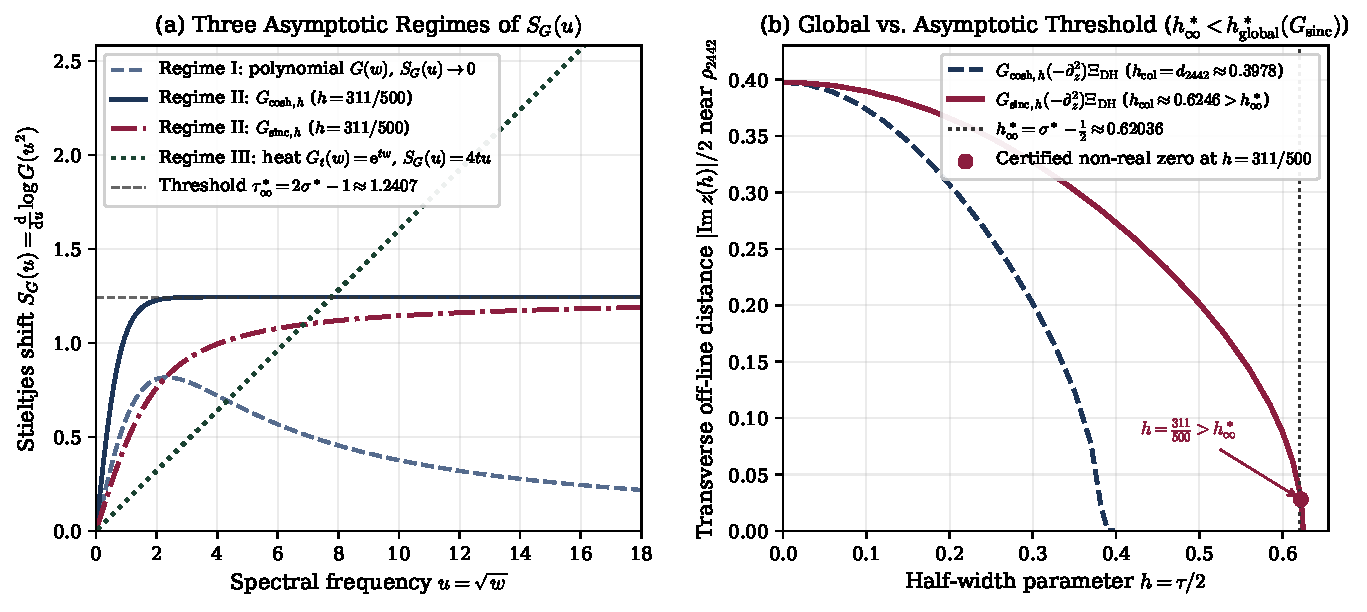
\includegraphics[width=0.98\textwidth]{../figures/fig2_polya_schur_sinc_vs_cosh.pdf}
  \caption{(a) Stieltjes logarithmic-derivative profiles $S_G(u)$ across Regimes~I, II, and~III relative to $\tau_\infty^* = 2\sigma^* - 1$. (b) Transverse off-line ordinate $|\Imop z(h)|/2$ near $\rho_{2442}$ under $G_{\mathrm{cosh},h}$ versus $G_{\mathrm{sinc},h}$, showing certified persistence past $h_\infty^* = \sigma^* - \frac{1}{2}$ across $[\sigma^* - \frac{1}{2}, 311/500]$.}
  \label{fig:stieltjes-sinc}
\end{figure}

\section{Shifted Gauss--Weierstrass Asymptotics and Strict Upper Bound}
\label{sec:upper-bound}

For $G_t(w) = \ee^{tw}$, de~Bruijn's hyperbola and strip theorems govern zero contraction under the backward heat semigroup.

\begin{lemma}[{de~Bruijn \cite[Thms.~12 and~13]{debruijn1950}}]
\label{lem:debruijn-strip}
Let $F(z)$ be a real-even entire function of genus~$0$ or~$1$ whose zeros all satisfy $|\Imop z| \le \Delta_0$.
\begin{enumerate}[label=\textup{(\roman*)},leftmargin=2.0em]
  \item For every $t > 0$, all zeros of $\ee^{-t\partial_z^2}F(z)$ satisfy $|\Imop z| \le \sqrt{\max(0, \Delta_0^2 - 2t)}$; in particular, $\Lambda_{\mathrm{DH}} \le 2(\sigma^* - \frac{1}{2})^2$.
  \item If $x_* \in \R$ and $\widetilde{\Delta} \ge 0$ are such that every zero $z_\rho$ of $F$ satisfies $(\Imop z_\rho)^2 - (\Reop z_\rho - x_*)^2 \le \widetilde{\Delta}^2$, then every zero $z$ of $\ee^{-t\partial_z^2}F(z)$ on the vertical line $\Reop z = x_*$ satisfies $(\Imop z)^2 \le \max(0, \widetilde{\Delta}^2 - 2t)$.
\end{enumerate}
\end{lemma}

To sharpen Lemma~\ref{lem:debruijn-strip}(i) to a \emph{strict} inequality $\Lambda_{\mathrm{DH}} < 2(\sigma^* - \frac{1}{2})^2$, we prove via the half-line folding \eqref{eq:boxed-folding} that for every $t > 0$, $H_t^{\mathrm{DH}}(z)$ has only real, simple zeros above an explicit closed-form height $\gamma_0(t)$, avoiding the incomplete-Gamma boundary-saddle transition required in Riemann--Siegel heat-kernel expansions \cite{polymath2019}. We first state the two elementary Dirichlet bounds proved in Appendix~\ref{app:analytic-constants}.

\begin{lemma}[Explicit Abel and Dirichlet-Tail Bounds]
\label{lem:abel-dirichlet}
For all $\tau \ge 100$ and $v \ge 0$, $|\mathcal{D}_{\mathrm{DH}}(\frac{1}{2} + v + \ii\tau)| \le 4\tau^{1/2}$. Moreover, for all $\tau \in \R$ and $u \ge \frac{5}{4}$, $\sum_{n=2}^{\infty} |a_{\mathrm{DH}}(n)|n^{-1/2 - u} < \frac{1}{2}$, so $\Reop\mathcal{D}_{\mathrm{DH}}(\frac{1}{2} + u + \ii\tau) > \frac{1}{2}$ and $|\mathcal{D}_{\mathrm{DH}}(\frac{1}{2} + u + \ii\tau)| < \frac{3}{2}$.
\end{lemma}

\begin{proposition}[Explicit Asymptotic Real-Rootedness and Simplicity for $H_t^{\mathrm{DH}}$]
\label{prop:asymptotic-simplicity}
Fix $t > 0$ and set $\Delta := \sigma^* - \frac{1}{2} < \frac{5}{8}$. Define the explicit closed-form cutoff height
\begin{equation}
  \gamma_0(t) := \max\!\left(400 + 64t^3,\; \frac{2\pi}{5}\exp\!\left(\frac{4}{t}\Bigl(\Delta + 5 + 6\sqrt{t} + 2t\Bigr)\right)\right).
  \label{eq:gamma0-cutoff}
\end{equation}
Then for all $|\gamma| \ge \gamma_0(t)$, $H_t^{\mathrm{DH}}(2\gamma - 2\ii\delta) \ne 0$ for every $\delta \ne 0$, and every real zero of $H_t^{\mathrm{DH}}(x)$ in $|x| \ge 2\gamma_0(t)$ is simple.
\end{proposition}

\begin{proof}
By evenness and Lemma~\ref{lem:debruijn-strip}(i), it suffices to consider $\gamma \ge \gamma_0(t)$ and $|\delta| \le \Delta$. In \eqref{eq:boxed-folding}, fix any $\eta \in [-\Delta, \Delta]$ and deform the ray $v \in [0,\infty)$ to $\mathcal{V}_\theta \cup \mathcal{C}_\theta$, where $\mathcal{V}_\theta := \{\ii y : 0 \le y \le \theta\}$, $\mathcal{C}_\theta := \{u + \ii\theta : u \ge 0\}$, and $\theta := \frac{\pi t}{8}$; this contour shift is justified pre-move because $\xi_{\mathrm{DH}}$ is entire and $|\ee^{-(u+\ii y-\eta)^2/t}\xi_{\mathrm{DH}}(\frac{1}{2}+u+\ii(\gamma+y))| \ll_{\gamma,\theta} \ee^{-u^2/(2t)} \to 0$ as $u \to +\infty$ uniformly for $y \in [0,\theta]$. Set $\tilde{\gamma} := \gamma + \theta > \gamma$ and $K_0(\gamma,\eta) := \ee^{\frac{\pi^2 t}{64} + \ii\frac{\pi}{4}\eta}\Gamma_{\mathrm{DH}}(\frac{1}{2} + \ii\tilde{\gamma}) \ne 0$. Along $v = u + \ii\theta$, expanding $-(u + \ii\theta - \eta)^2/t = -\frac{(u-\eta)^2}{t} + \frac{\pi^2 t}{64} - \ii\frac{\pi}{4}(u - \eta)$ cancels the $+\ii\frac{\pi}{4}u$ Stirling phase of $\Gamma_{\mathrm{DH}}(\frac{1}{2} + u + \ii\tilde{\gamma}) / \Gamma_{\mathrm{DH}}(\frac{1}{2} + \ii\tilde{\gamma}) = (\frac{5\tilde{\gamma}}{2\pi})^{u/2}\ee^{\ii\frac{\pi}{4}u + E_{\mathrm{St}}(u,\tilde{\gamma})}$ identically, yielding
\begin{equation}
  \frac{\sqrt{\pi t}\,\ee^{-u_0^2/t + \eta^2/t}}{K_0(\gamma,\eta)}\,A_t(\gamma,\eta)
  = \int_{0}^{\infty} \ee^{-(u - u_0)^2/t + E_{\mathrm{St}}(u,\tilde{\gamma})}\,\mathcal{D}_{\mathrm{DH}}\!\left(\tfrac{1}{2} + u + \ii\tilde{\gamma}\right)\dd u + \mathcal{E}_{\mathcal{V}}(\gamma,\eta),
  \label{eq:shifted-A}
\end{equation}
where $u_0 = u_0(\gamma,\eta) := \eta + \frac{t}{4}\log\frac{5\tilde{\gamma}}{2\pi}$. Under \eqref{eq:gamma0-cutoff}, $u_0 > 5 + 6\sqrt{t} + 2t$ for all $\eta \in [-\Delta,\Delta]$. As proved in Appendix~\ref{app:analytic-constants}, Binet's digamma bound gives $|E_{\mathrm{St}}(u,\tilde{\gamma})| \le \frac{u^2 + 6u}{4\tilde{\gamma}}$ for all $u \ge 0$, so $|E_{\mathrm{St}}(u,\tilde{\gamma})| < \frac{1}{10}$ on $|u - u_0| \le 3\sqrt{t}$ (where $u > 5 > \frac{5}{4}$ and $\Reop(\ee^{E_{\mathrm{St}}}\mathcal{D}_{\mathrm{DH}}) \ge \ee^{-1/10}(\frac{1}{2}\cos\frac{1}{10} - \frac{3}{2}\sin\frac{1}{10}) > 0.31$), while the split left tail $[0, \frac{5}{4}] \cup [\frac{5}{4}, u_0 - 3\sqrt{t}]$, vertical segment $\mathcal{V}_\theta$, and right tail $u \ge u_0 + 3\sqrt{t}$ contribute less than $0.015\sqrt{\pi t}$ in modulus, leaving real part $> 0.29\sqrt{\pi t}$. Inserting $\frac{2}{t}(v - \eta) = (\frac{1}{2}\log\frac{5\tilde{\gamma}}{2\pi} + \ii\frac{\pi}{4}) + \frac{2}{t}(u - u_0)$ for $\partial_\eta A_t(\gamma,\eta)$ bounds the centered-moment remainder by $\frac{6.7}{\sqrt{t}} < \frac{1}{4}\log\frac{5\tilde{\gamma}}{2\pi}$ (Appendix~\ref{app:analytic-constants}), showing that $A_t(\gamma,\eta) \ne 0$ and
\begin{equation}
  \Reop\!\left(\frac{\partial_\eta A_t(\gamma,\eta)}{A_t(\gamma,\eta)}\right)
  \ge \frac{1}{4}\log\frac{5\tilde{\gamma}}{2\pi} > 1
  \qquad \forall\,\eta \in [-\Delta,\Delta].
  \label{eq:log-monotonicity}
\end{equation}
Consequently, for every $\delta \in (0, \Delta]$, integrating \eqref{eq:log-monotonicity} over $[-\delta, \delta]$ gives $\log|A_t(\gamma,\delta)| - \log|A_t(\gamma,-\delta)| = \int_{-\delta}^{\delta}\Reop(\partial_\eta A_t / A_t)\,\dd\eta > 0$, whence $|H_t^{\mathrm{DH}}(2\gamma - 2\ii\delta)| \ge |A_t(\gamma,\delta)| - |A_t(\gamma,-\delta)| > 0$. Finally, at $\delta = 0$, $H_t^{\mathrm{DH}}(2\gamma) = 2|A_t(\gamma,0)|\cos\Theta_t(\gamma)$ with $\Theta_t(\gamma) := \arg A_t(\gamma,0)$; dividing the second identity of \eqref{eq:boxed-folding} at $\delta = 0$ by $A_t(\gamma,0)$ and applying the explicit boundary ratio bound $< 10^{-2}$ from Appendix~\ref{app:analytic-constants} yields
\begin{equation}
  \Theta_t'(\gamma) = \Reop\!\left(\frac{\partial_\delta A_t(\gamma,0)}{A_t(\gamma,0)}\right) - \Reop\!\left(\frac{\xi_{\mathrm{DH}}(\frac{1}{2}+\ii\gamma)}{\sqrt{\pi t}\,A_t(\gamma,0)}\right)
  \ge \frac{1}{4}\log\frac{5\gamma}{2\pi} - 10^{-2} > 1 > 0,
  \label{eq:theta-prime-pos}
\end{equation}
so $\frac{\dd}{\dd\gamma}H_t^{\mathrm{DH}}(2\gamma) = \mp 2|A_t(\gamma,0)|\Theta_t'(\gamma) \ne 0$ at every real zero $\cos\Theta_t(\gamma) = 0$.
\end{proof}

\begin{theorem}[Strict Unconditional Upper Bound for $\Lambda_{\mathrm{DH}}$]
\label{thm:strict-upper-bound}
The de~Bruijn--Newman constant of $\Xi_{\mathrm{DH}}(z)$ satisfies the strict inequality
\begin{equation}
  \Lambda_{\mathrm{DH}} < 2\Bigl(\sigma^* - \tfrac{1}{2}\Bigr)^2 = 0.76969925830451198120\ldots
  \label{eq:strict-upper}
\end{equation}
\end{theorem}

\begin{proof}
Set $\Delta_0 := 2(\sigma^* - \frac{1}{2})$ and fix $t_1 := \frac{1}{2} < \frac{1}{2}\Delta_0^2 = 2(\sigma^* - \frac{1}{2})^2$. By Proposition~\ref{prop:asymptotic-simplicity}, all zeros of $H_{t_1}^{\mathrm{DH}}(z)$ in $|\Reop z| \ge 2\gamma_0(t_1)$ are real, so $H_{t_1}^{\mathrm{DH}}$ possesses at most finitely many non-real zeros, all confined to $|\Reop z| < 2\gamma_0(t_1)$. If $H_{t_1}^{\mathrm{DH}}$ has no non-real zeros, then $\Lambda_{\mathrm{DH}} \le t_1 < 2(\sigma^* - \frac{1}{2})^2$. Otherwise, $Y_1 := \max\{|\Imop w| : H_{t_1}^{\mathrm{DH}}(w) = 0\} > 0$ is attained at some $w_* = x_* + \ii y_*$ with $|x_*| < 2\gamma_0(t_1)$.

We verify first that every individual zero $z_\rho = x_\rho + \ii y_\rho$ of $\Xi_{\mathrm{DH}}(z)$ satisfies $|y_\rho| < \Delta_0$ strictly. Zeros with $0 \le \Reop\rho \le 1$ satisfy $|y_\rho| \le 1 < \Delta_0$. For $\Reop\rho = \sigma > 1$ (and symmetrically $\Reop\rho < 0$), $\mathcal{D}_{\mathrm{DH}}(\sigma + \ii\gamma) = 0$ implies $L(\sigma+\ii\gamma, \overline{\chi_5})/L(\sigma+\ii\gamma, \chi_5) = \ee^{-2\ii(\frac{\pi}{2} - \arctan\kappa)}$. In the Euler product, primes $p \equiv 1,4 \pmod{5}$ cancel identically, while for each $p \equiv 2,3 \pmod{5}$ the M\"obius factor $\frac{1 + w_p}{1 - w_p}$ ($w_p := \chi_5(p)p^{-\sigma-\ii\gamma}$, $|w_p| = p^{-\sigma}$) maps $|w| = p^{-\sigma}$ onto the circle over $[\frac{1 - p^{-\sigma}}{1 + p^{-\sigma}}, \frac{1 + p^{-\sigma}}{1 - p^{-\sigma}}]$, giving $|\arg\frac{1+w_p}{1-w_p}| \le \arcsin(\frac{2p^{-\sigma}}{1 + p^{-2\sigma}}) = 2\arctan(p^{-\sigma})$, with equality if and only if $\Reop w_p = 0$ (i.e., $p^{-\ii\gamma} = \pm 1$). Since $\frac{\log 3}{\log 2} \notin \Q$, equality cannot hold simultaneously for $p = 2$ and $p = 3$ at any $\gamma \in \R$, forcing $\sigma < \sigma^*$ and $|y_\rho| < \Delta_0$.

Now set $R := 2\gamma_0(t_1) + \Delta_0 + 1$. The finitely many zeros of $\Xi_{\mathrm{DH}}$ in $|\Reop z_\rho| \le R$ satisfy $\Delta_R := \max_{|\Reop z_\rho| \le R} |\Imop z_\rho| < \Delta_0$, while every zero with $|\Reop z_\rho| > R$ satisfies $|\Reop z_\rho - x_*| > \Delta_0 + 1 > |\Imop z_\rho|$, so $(\Imop z_\rho)^2 - (\Reop z_\rho - x_*)^2 < 0$. Hence every zero of $\Xi_{\mathrm{DH}}$ satisfies $(\Imop z_\rho)^2 - (\Reop z_\rho - x_*)^2 \le \Delta_R^2 < \Delta_0^2$. Lemma~\ref{lem:debruijn-strip}(ii) at $\Reop z = x_*$ yields $Y_1^2 \le \max(0, \Delta_R^2 - 2t_1)$, and applying Lemma~\ref{lem:debruijn-strip}(i) to $H_{t_1 + t_2}^{\mathrm{DH}} = \ee^{-t_2\partial_z^2}H_{t_1}^{\mathrm{DH}}$ with $t_2 := \frac{1}{2}Y_1^2$ gives $\Lambda_{\mathrm{DH}} \le t_1 + \frac{1}{2}Y_1^2 \le \max(t_1, \frac{1}{2}\Delta_R^2) < \frac{1}{2}\Delta_0^2 = 2(\sigma^* - \frac{1}{2})^2$.
\end{proof}

\section{Interval-Certified Separation $\Lambda_\zeta \le 1/5 < 1153/5000 < \Lambda_{\mathrm{DH}}$}
\label{sec:lower-bound}

\subsection{Rigorous theta-kernel truncation and Interval--Newton certificates}
\label{subsec:interval-newton}

To establish unconditional lower bounds on $\Lambda_{\mathrm{DH}}$ free of quadrature aliasing or uncertified root-tracking heuristics, we evaluate $H_t^{\mathrm{DH}}(z) = 2\int_{0}^{\infty}\ee^{tu^2}\Phi_{\mathrm{DH}}(u)\cos(zu)\,\dd u$ and $\partial_z H_t^{\mathrm{DH}}(z)$ directly in arbitrary-precision complex ball arithmetic \cite{johansson2017} on a finite interval $[0, U]$ with certified analytical remainder balls.

\begin{lemma}[Rigorous Theta-Kernel Truncation and Second-Derivative Bounds]
\label{lem:theta-truncation}
Let $0 \le t \le \frac{1}{4}$, $2 \le U \le \frac{5}{2}$, $N \ge 25$, and $|y| \le 1$, where $y = \Imop z$. Approximating $\Phi_{\mathrm{DH}}(u)$ on $[0, U]$ by $\Phi_{\mathrm{DH}}^{(<N)}(u) := 4\ee^{3u}\sum_{n=1}^{N-1} n\,a_{\mathrm{DH}}(n)\,\ee^{-\pi n^2\ee^{4u}/5}$ incurs a total truncation error bounded for $k \in \{0, 1, 2\}$ ($\partial_z^k H_t^{\mathrm{DH}}$) by
\begin{equation}
  \left|\partial_z^k H_t^{\mathrm{DH}}(z) - 2\int_{0}^{U} \ee^{tu^2}\Phi_{\mathrm{DH}}^{(<N)}(u)\,\partial_z^k\cos(zu)\,\dd u\right|
  \le E_1(U,N,k,|y|) + E_2(U),
  \label{eq:theta-tail-bound}
\end{equation}
where $r_N := \ee^{-\pi N/5}$, $E_1(U,N,k,|y|) := 8 U^{k+1}\ee^{t U^2 + (3+|y|)U}\frac{r_N^N(N - (N-1)r_N)}{(1 - r_N)^2}$, and $E_2(U) := \frac{40}{\pi}\ee^{-4U - \frac{\pi}{10}\ee^{4U}}$. Moreover, on any closed box $B$ with $\max_{z \in B}|\Imop z| \le y_{\max} \le 1$, one has
\begin{equation}
  \sup_{z \in B}\left|\partial_z^2 H_t^{\mathrm{DH}}(z)\right|
  \le 4N(N-1)U^3 \ee^{t U^2 + 3U}\cosh(U y_{\max}) + E_1(U,N,2,y_{\max}) + E_2(U).
  \label{eq:m2-bound}
\end{equation}
\end{lemma}

The proof of Lemma~\ref{lem:theta-truncation} is given in Appendix~\ref{app:truncation-bounds}. Combining Lemma~\ref{lem:theta-truncation} with complex Interval--Newton contraction $N(B) := z_0 - H_t^{\mathrm{DH}}(z_0) / [H_t^{\mathrm{DH}\prime}(z_0) + (B - z_0)M_2(B)]$ yields our certified separation theorem.

\begin{theorem}[Interval-Certified Lower Bounds and Separation from $\Lambda_\zeta$]
\label{thm:certified-lower}
Let $B(z_0, r) := \{z \in \C : |\Reop(z - z_0)| \le r,\; |\Imop(z - z_0)| \le r\}$.
\begin{enumerate}[label=\textup{(\roman*)},leftmargin=2.0em]
  \item At exact rational $t = \frac{1}{5} = 0.2$, $H_{1/5}^{\mathrm{DH}}(z)$ possesses two independent certified simple non-real zeros in $\Imop z < 0$: one inside $B(z_{240}^{(1/5)}, 10^{-90})$ originating from $\rho_{240}$, and a second inside $B(z_{531}^{(1/5)}, 10^{-193})$ originating from $\rho_{531}$ (Table~\ref{tab:certificates}).
  \item At exact rational $t = \frac{1153}{5000} = 0.2306$, $H_{1153/5000}^{\mathrm{DH}}(z)$ possesses a certified simple non-real zero inside $B(z_{240}^{(1153/5000)}, 10^{-94})$ with $\Imop z < -3.83 \times 10^{-3} < 0$ (Table~\ref{tab:certificates}).
\end{enumerate}
By Lemma~\ref{lem:debruijn-strip}(i) and Platt and Trudgian's unconditional bound $\Lambda_\zeta \le \frac{1}{5}$ \cite{platt2021}, it follows unconditionally that $\Lambda_\zeta \le \frac{1}{5} < \frac{1153}{5000} < \Lambda_{\mathrm{DH}}$.
\end{theorem}

\begin{proof}
Using 640-bit, 704-bit, and 1350-bit \texttt{FLINT/Arb} Gauss--Legendre ball quadrature (\texttt{acb.integral} \cite{johansson2017}) with the analytical remainder enclosures of Lemma~\ref{lem:theta-truncation}, our verification suite evaluates $H_t^{\mathrm{DH}}(z_0)$, $\partial_z H_t^{\mathrm{DH}}(z_0)$, and \eqref{eq:m2-bound} at each rational parameter $t$ and midpoint $z_0$ listed in Table~\ref{tab:certificates}. In every case, $0 \notin \partial_z H_t^{\mathrm{DH}}(z_0) + (B - z_0)M_2(B)$, $N(B)$ lies strictly inside $\operatorname{int}(B)$, and $\sup_{w \in N(B)} \Imop w < 0$. By Brouwer's fixed-point theorem and the Argument Principle, $H_t^{\mathrm{DH}}$ has a unique simple zero in $B$, which is strictly non-real. If $H_{t_0}^{\mathrm{DH}}$ had only real zeros for some $t_0 \le \frac{1153}{5000}$, then Lemma~\ref{lem:debruijn-strip}(i) applied to $H_{1153/5000}^{\mathrm{DH}} = \ee^{-(1153/5000 - t_0)\partial_z^2}H_{t_0}^{\mathrm{DH}}$ would force all zeros at $t = \frac{1153}{5000}$ to be real, contradicting~(ii); openness of simple non-real zeros in $t$ gives the strict inequality $\Lambda_{\mathrm{DH}} > \frac{1153}{5000}$.
\end{proof}

\begin{table}[t]
  \centering
  \caption{Summary of \texttt{FLINT/Arb} ball-arithmetic enclosures and Interval--Newton contractions ($N(B) \subset \operatorname{int}(B)$) verified by \nolinkurl{verify_paper15_debruijn_newman_dh.py}.}
  \label{tab:certificates}
  \footnotesize
  \renewcommand{\arraystretch}{1.18}
  \setlength{\tabcolsep}{4.8pt}
  \begin{tabular}{@{}lllc@{}}
    \toprule
    Target / Witness & Param. & Certified Midpoint / Enclosure (16 digits shown) & Radius $r$ \\
    \midrule
    Bohr supremum $\sigma^*$ & IVT & $1.1203624981833251$ & $10^{-32}$ \\
    $G_{\mathrm{sinc}}$ ($\rho_{2442}$, 384-bit) & $h = \frac{311}{500}$ & $4884.886654191757 - 0.0560046288608581\,\ii$ & $10^{-45}$ \\
    $G_{\mathrm{sinc}}$ continuum & $[\frac{310}{500}, \frac{311}{500}]$ & $64$ overlapping balls $H_k$, $\Imop N(B_k, H_k) < 0$ & $1.5\times 10^{-3}$ \\
    $H_t^{\mathrm{DH}}$ ($\rho_1$, 384-bit) & $t = \frac{22}{125}$ & $171.2354942735178 - 0.0317958184889241\,\ii$ & $10^{-48}$ \\
    $H_t^{\mathrm{DH}}$ ($\rho_{240}$, 640-bit) & $t = \frac{1}{5}$ & $480.7066441211221 - 0.2501436731312467\,\ii$ & $10^{-90}$ \\
    $H_t^{\mathrm{DH}}$ ($\rho_{531}$, 1350-bit) & $t = \frac{1}{5}$ & $1062.459584704108 - 0.0505424679933243\,\ii$ & $10^{-193}$ \\
    $H_t^{\mathrm{DH}}$ ($\rho_{240}$, 704-bit) & $t = \frac{1153}{5000}$ & $480.6902350136200 - 0.0038371695655869\,\ii$ & $10^{-94}$ \\
    \bottomrule
  \end{tabular}
\end{table}

\begin{figure}[t]
  \centering
  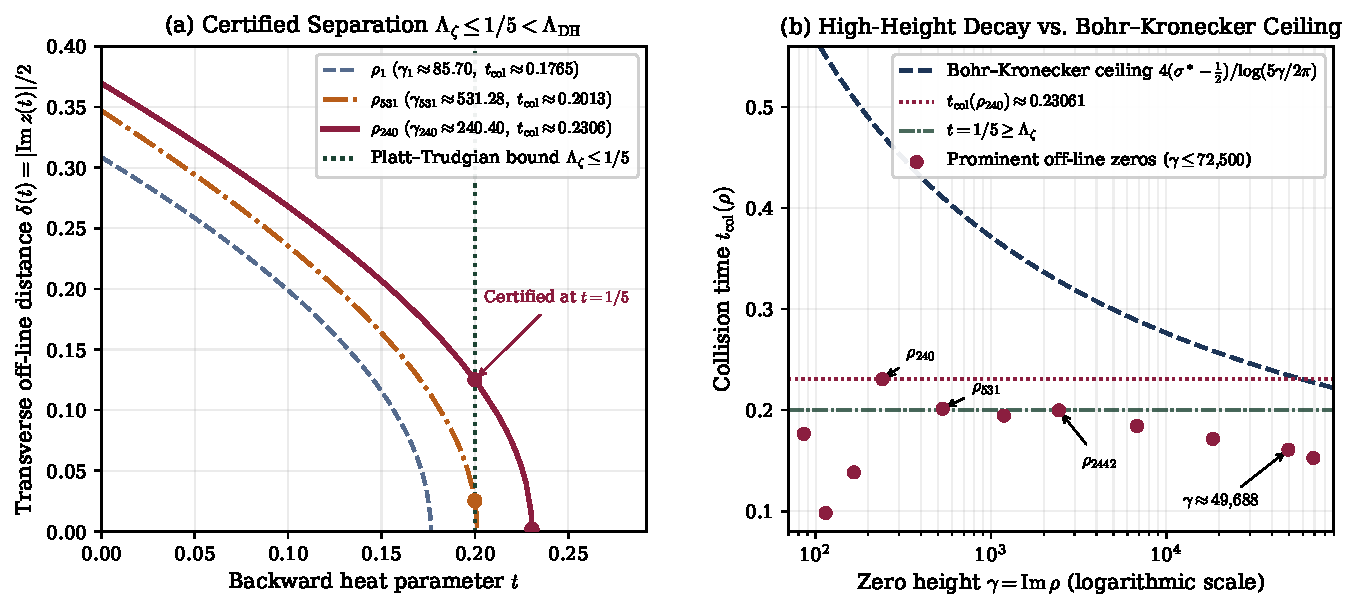
\includegraphics[width=0.98\textwidth]{../figures/fig1_heat_flow_separation_witnesses.pdf}
  \caption{(a) Transverse off-line distance $\delta(t) = |\Imop z(t)|/2$ under backward heat flow for $\rho_1$, $\rho_{240}$, and $\rho_{531}$, showing certified non-real witnesses at $t = 1/5 \ge \Lambda_\zeta$ and $t = 1153/5000 = 0.2306$. (b) Numerical survey of prominent off-line collision times up to $\gamma = 72{,}500$ compared with the asymptotic Bohr--Kronecker ceiling $4(\sigma^* - \frac{1}{2})/\log(\frac{5\gamma}{2\pi})$.}
  \label{fig:heat-witnesses}
\end{figure}

\subsection{Numerical high-height collision survey versus certified theorems}
\label{subsec:numerical-survey}

We strictly distinguish the ball-certified theorems in Table~\ref{tab:certificates} from exploratory numerical computations:
\begin{enumerate}[label=\textup{(\arabic*)},leftmargin=2.0em]
  \item \emph{Oscillation aliasing in non-interval quadrature:} Near the first off-line zero $\rho_1 \approx 0.808517 + 85.699348\,\ii$ ($z \approx 171.40 - 0.6170\,\ii$), $\cos(zu)$ undergoes roughly $60$ oscillations on $[0, 2.25]$. Uncertified adaptive Gauss--Legendre quadrature (\texttt{mpmath.quad} at default subdivision) aliases across sign changes and reports a spurious coalescence near $t \approx 0.14194$, whereas the 384-bit \texttt{FLINT/Arb} certificate in Table~\ref{tab:certificates} proves $\Imop z_1(\frac{22}{125}) < 0$ at $t = \frac{22}{125} = 0.176$ (high-precision collision refinement: $t_{\mathrm{col}}(\rho_1) \approx 0.1765053782$).
  \item \emph{High-precision collision coordinates and high-height scan:} Scalar Newton refinement on $(H_t^{\mathrm{DH}}, \partial_z H_t^{\mathrm{DH}}) = (0,0)$ locates the coalescence of $\rho_{240}$ at $t_{\mathrm{col}}(\rho_{240}) \approx 0.2306073618964546$ ($x_{\mathrm{col}} \approx 480.6902310425$)---matching the uncertified six-digit value $0.230607$ noted heuristically in \cite{mcgreevy2026}---and that of $\rho_{531}$ at $t_{\mathrm{col}}(\rho_{531}) \approx 0.20127583$. An exploratory scan of off-line zeros of $\mathcal{D}_{\mathrm{DH}}(s)$ up to $\gamma = 72{,}500$ (Figure~\ref{fig:heat-witnesses}(b)) detects no collision exceeding $t_{\mathrm{col}}(\rho_{240})$: although deeper real parts occur at higher ordinates (such as $\rho_{2442}$ with $\Reop\rho \approx 0.89775$ and $t_{\mathrm{col}} \approx 0.19973$, or $\gamma \approx 49{,}688.34$ with $\Reop\rho \approx 0.93187$ and $t_{\mathrm{col}} \approx 0.1609$), Stirling's logarithmic factor $\frac{1}{2}\log\frac{5\gamma}{2\pi}$ accelerates transverse heat speed according to the asymptotic ceiling $t_{\mathrm{col}}(\rho) \lesssim \frac{4(\sigma^* - 1/2)}{\log(5\gamma/(2\pi))} \to 0$ implied by Proposition~\ref{prop:asymptotic-simplicity}. Whether $\Lambda_{\mathrm{DH}}$ coincides with $t_{\mathrm{col}}(\rho_{240})$ remains an open finite-box verification problem.
\end{enumerate}

\section{Scope, Limitations, and Open Questions}
\label{sec:conclusion}

Theorem~\ref{thm:main} demonstrates that for self-dual Dirichlet series without an Euler product, P\'olya--Schur differential multipliers exhibit two distinct phenomena absent under the Riemann Hypothesis: an infinite-height phase transition governed by the Stieltjes logarithmic derivative $S_G(u)$ relative to $2\sigma^* - 1$ (sensitive to root-gap regularity even when $\rho(G) \in (1/2,1)$), and a strict gap between the infinite-height Kronecker threshold $h_\infty^* = \sigma^* - \frac{1}{2}$ and global real-rootedness for strip-averaging multipliers such as $G_{\mathrm{sinc},h}$. Closing the rigorous interval $\frac{1153}{5000} < \Lambda_{\mathrm{DH}} < 2(\sigma^* - \frac{1}{2})^2$ to arbitrary precision reduces, via Proposition~\ref{prop:asymptotic-simplicity}, to a finite two-dimensional argument-principle box cover up to height $\gamma_0(t)$ once $\gamma_0(t)$ is optimized via stationary-phase Dirichlet sums.

\appendix

\section{Proofs of Explicit Analytic Constants and Gaussian Tail Bounds}
\label{app:analytic-constants}

\begin{proof}[Proof of Lemma~\ref{lem:abel-dirichlet}]
Set $S(N) := \sum_{n=1}^{N} a_{\mathrm{DH}}(n)$. Because $a_{\mathrm{DH}}(n+5) = a_{\mathrm{DH}}(n)$ and $\sum_{r=1}^{5} a_{\mathrm{DH}}(r) = 1 + \kappa - \kappa - 1 + 0 = 0$, checking $N \equiv 1,2,3,4,0 \pmod{5}$ gives $\max_{N \ge 1}|S(N)| = 1 + \kappa < 1.2841$. Fix $\tau \ge 100$, $v \ge 0$, set $\sigma := \frac{1}{2} + v \ge \frac{1}{2}$, and choose $M := \lfloor\tau\rfloor \ge 100$. Splitting $\mathcal{D}_{\mathrm{DH}}(\sigma + \ii\tau) = \sum_{n=1}^{M} a_{\mathrm{DH}}(n)n^{-\sigma-\ii\tau} + \sum_{n=M+1}^{\infty} a_{\mathrm{DH}}(n)n^{-\sigma-\ii\tau}$, the prefix satisfies
\begin{equation}
  \begin{aligned}
    \left|\sum_{n=1}^{M} a_{\mathrm{DH}}(n)n^{-\sigma-\ii\tau}\right|
    &\le 2(1+\kappa)\sum_{m=0}^{\lfloor (M-1)/5\rfloor} (5m+1)^{-1/2} \\
    &\le 2(1+\kappa)\Bigl(1 + \frac{2}{5}(\sqrt{\tau} - 1)\Bigr)
    \le 2(1+\kappa)(0.46\tau^{1/2}) < 1.19\,\tau^{1/2},
  \end{aligned}
  \label{eq:abel-prefix}
\end{equation}
since $\sum_{r=1}^{5}|a_{\mathrm{DH}}(5m+r)| = 2(1+\kappa)$ and $\frac{3}{5} + \frac{2}{5}\sqrt{\tau} \le 0.46\sqrt{\tau}$ for $\tau \ge 100$. Summing the tail $n \ge M+1$ by parts yields the remainder $-S(M)(M+1)^{-\sigma-\ii\tau}$ plus $(\sigma + \ii\tau)\int_{M+1}^{\infty} S(\lfloor x\rfloor)x^{-\sigma-1-\ii\tau}\,\dd x$. Since $M + 1 = \lfloor\tau\rfloor + 1 > \tau \ge 100$, for $\sigma \le 19\tau^{1/2}/20$ we have $|\sigma + \ii\tau| \le \tau\sqrt{1 + \frac{361}{400\tau}} \le 1.005\,\tau$ and $\int_{M+1}^{\infty} x^{-3/2}\,\dd x = 2(M+1)^{-1/2} < 2\tau^{-1/2}$, so the tail is at most $(1+\kappa)\tau^{-1/2} + 1.005(1+\kappa)\cdot 2\tau^{1/2} < 2.71\,\tau^{1/2}$, giving $|\mathcal{D}_{\mathrm{DH}}(\sigma+\ii\tau)| < (1.19 + 2.71)\tau^{1/2} = 3.90\,\tau^{1/2} < 4\tau^{1/2}$. When $\sigma > 19\tau^{1/2}/20 \ge \frac{19}{2}$, $|\mathcal{D}_{\mathrm{DH}}(\sigma+\ii\tau)| \le \zeta(19/2) < 1.002 < 4\tau^{1/2}$. Finally, for $u \ge \frac{5}{4}$ ($\sigma = \frac{1}{2} + u \ge \frac{7}{4}$), monotonicity in $\sigma$ and Hurwitz evaluation at $\sigma = \frac{7}{4}$ give $5^{-7/4}[\zeta(\frac{7}{4},\frac{1}{5}) - 5^{7/4} + \kappa(\zeta(\frac{7}{4},\frac{2}{5}) + \zeta(\frac{7}{4},\frac{3}{5})) + \zeta(\frac{7}{4},\frac{4}{5})] = 0.41770137\ldots < \frac{1}{2}$ for $\sum_{n=2}^{\infty} |a_{\mathrm{DH}}(n)|n^{-7/4}$, whence $\Reop\mathcal{D}_{\mathrm{DH}} > 1 - \frac{1}{2} = \frac{1}{2}$ and $|\mathcal{D}_{\mathrm{DH}}| < 1 + \frac{1}{2} = \frac{3}{2}$.
\end{proof}

\begin{proof}[Completion of Binet and tail bounds in Proposition~\ref{prop:asymptotic-simplicity}]
Write $z_0 := \frac{3}{4} + \frac{\ii\tilde{\gamma}}{2}$, so $|z_0| > \frac{\tilde{\gamma}}{2} \ge 200$. By Binet's second integral formula, $\log\Gamma(z_0 + \frac{u}{2}) - \log\Gamma(z_0) - \frac{u}{2}\log z_0 = \int_{0}^{u/2}[\psi(z_0+w) - \log(z_0+w) + \log(1 + \frac{w}{z_0})]\,\dd w$. Since $|\psi(z) - \log z + \frac{1}{2z}| \le \frac{1}{6|z|^2}$ on $\Reop z > 0$ and $|\log(1 + \frac{w}{z_0})| \le \frac{w}{|z_0|}$ for all $w \ge 0$, we obtain $|\log\frac{\Gamma(z_0 + u/2)}{\Gamma(z_0)} - \frac{u}{2}\log z_0| \le \frac{u^2 + 3u}{8|z_0|}$. Combined with $|\frac{u}{2}(\log z_0 - \log\frac{\ii\tilde{\gamma}}{2})| = \frac{u}{2}|\log(1 - \frac{3\ii}{2\tilde{\gamma}})| \le \frac{3u}{4\tilde{\gamma}}$, this gives $|E_{\mathrm{St}}(u,\tilde{\gamma})| \le \frac{u^2 + 6u}{4\tilde{\gamma}}$ for all $u \ge 0$. Set $X := \log\frac{5\tilde{\gamma}}{2\pi}$. By \eqref{eq:gamma0-cutoff}, $\frac{t}{4}X > \Delta + 5 + 6\sqrt{t} + 2t$ and $\tilde{\gamma} > \max(64t^3, \ee^X) \ge (64t^3)^{2/3}(\ee^X)^{1/3} = 16 t^2 \ee^{X/3}$. Since $u_0 + 3\sqrt{t} = \frac{t}{4}X + \eta + 3\sqrt{t} \in (5, \frac{t}{2}X)$, on $u \in [0, u_0 + 3\sqrt{t}]$ we have $|E_{\mathrm{St}}(u,\tilde{\gamma})| < \frac{\frac{11}{20}t^2 X^2}{64 t^2 \ee^{X/3}} = \frac{11}{1280}X^2\ee^{-X/3} \le \frac{11}{1280}\cdot 36\ee^{-2} < 0.042 < \frac{1}{10}$. On the right tail $u \ge u_0 + 3\sqrt{t}$, $\frac{u^2 + 6u}{4\tilde{\gamma}} \le \frac{(u_0 + 3)^2 + (u - u_0)^2}{\tilde{\gamma}} < \frac{1}{10} + \frac{(u - u_0)^2}{2t}$ (as $\tilde{\gamma} > 400 + 64t^3 > 2t$), so Lemma~\ref{lem:abel-dirichlet} bounds the right tail by $\frac{3}{2}\ee^{1/10}\int_{3\sqrt{t}}^{\infty}\ee^{-y^2/(2t)}\,\dd y < 0.01\sqrt{\pi t}$. Splitting the left tail at $u = \frac{5}{4}$, on $[\frac{5}{4}, u_0 - 3\sqrt{t}]$ Lemma~\ref{lem:abel-dirichlet} gives $|\mathcal{D}_{\mathrm{DH}}| < \frac{3}{2}$ and $|E_{\mathrm{St}}| < \frac{1}{10}$, bounded by $\frac{3}{2}\ee^{1/10}\int_{3\sqrt{t}}^{\infty}\ee^{-y^2/t}\,\dd y < 10^{-4}\sqrt{\pi t}$. On $[0, \frac{5}{4}]$ and on $\mathcal{V}_\theta = \{\ii y : 0 \le y \le \theta\}$, we have $u_0 - \frac{5}{4} > \max(\frac{15}{4} + 6\sqrt{t} + 2t,\; \frac{1}{6}t X)$, so splitting $(u_0 - \frac{5}{4})^2 = (\frac{17}{20} + \frac{3}{20})(u_0 - \frac{5}{4})^2$ gives $\frac{(u_0 - 5/4)^2}{t} > \frac{17}{32}X + \frac{2.1}{t} + \frac{6.75}{\sqrt{t}} + 5.4 + 0.6t$. Combining $|\mathcal{D}_{\mathrm{DH}}| \le 4\tilde{\gamma}^{1/2} < 4.52\ee^{X/2}$ with $|\Gamma_{\mathrm{DH}}(\frac{1}{2}+\ii(\gamma+y))/\Gamma_{\mathrm{DH}}(\frac{1}{2}+\ii\tilde{\gamma})| \le \ee^{\frac{\pi}{4}(\theta - y) + 0.01}$ and $\frac{\pi^2 t}{64} < 0.16 t$ bounds the $[0, \frac{5}{4}]$ integral by $5\tilde{\gamma}^{1/2}\ee^{0.01 - (u_0 - 5/4)^2/t} < 10^{-3}\sqrt{\pi t}$, $|\mathcal{E}_{\mathcal{V}}| \le \frac{\pi t}{2}\tilde{\gamma}^{1/2}\ee^{0.01 - u_0^2/t + \pi^2 t/64} < 10^{-3}\sqrt{\pi t}$, and $|\xi_{\mathrm{DH}}(\frac{1}{2}+\ii\gamma)/(\sqrt{\pi t}\,A_t(\gamma,0))| \le 4\tilde{\gamma}^{1/2}\ee^{0.01 - u_0^2/t + \pi^2 t/64}/(0.29\sqrt{\pi t}) < 10^{-2}$. Finally, for $\partial_\eta A_t(\gamma,\eta)$, integrating $\frac{2|u - u_0|}{t}\ee^{-(u-u_0)^2/t}$ over $[\frac{5}{4}, u_0 + 3\sqrt{t}]$ contributes at most $3\ee^{1/10} < \frac{1.88}{\sqrt{t}}\sqrt{\pi t}$ (with $< \frac{0.06}{\sqrt{t}}\sqrt{\pi t}$ from the remaining pieces via $\ee^{-X/32}$), and dividing by $0.29\sqrt{\pi t}$ gives $< \frac{6.7}{\sqrt{t}} < \frac{\Delta + 5}{t} + \frac{6}{\sqrt{t}} + 2 < \frac{1}{4}X = \frac{1}{4}\log\frac{5\tilde{\gamma}}{2\pi}$, establishing \eqref{eq:log-monotonicity} and \eqref{eq:theta-prime-pos}.
\end{proof}

\section{Ball-Arithmetic Truncation Enclosures}
\label{app:truncation-bounds}

\begin{proof}[Proof of Lemma~\ref{lem:theta-truncation} and Cauchy bound in Theorem~\ref{thm:sinc-separation}]
For $n \ge N \ge 25$ and $u \in [0, U]$, we have $\ee^{4u} \ge 1$ and $n^2 \ge Nn$, so $\ee^{-\pi n^2\ee^{4u}/5} \le r_N^n$ with $r_N = \ee^{-\pi N/5} < 10^{-6}$. Since $|a_{\mathrm{DH}}(n)| \le 1$ ($\kappa < 0.285 < 1$), summing $\sum_{n=N}^{\infty} n\,r_N^n = \frac{r_N^N(N - (N-1)r_N)}{(1 - r_N)^2}$ and using $|\partial_z^k\cos(zu)| \le u^k\ee^{|y|u} \le U^k\ee^{|y|U}$ over $[0, U]$ gives $E_1(U,N,k,|y|)$. For $u \ge U \ge 2$, $\ee^{4u} \ge \ee^8 > 2980$, so $\sum_{n=1}^{\infty} n\,\ee^{-\pi n^2\ee^{4u}/5} \le 2\ee^{-\pi\ee^{4u}/5}$; moreover, for $0 \le t \le \frac{1}{4}$ and $|y| \le 1$, $t u^2 + (3 + |y|)u + k\log u \le \frac{u^2}{4} + 6u \le \frac{\pi}{10}\ee^{4u} - 4u$ for all $u \ge 2$. Hence the integrand on $[U,\infty)$ is bounded by $16\ee^{-4u - \frac{\pi}{10}\ee^{4u}} \le \frac{40}{\pi}\ee^{-4U}\cdot \frac{2\pi}{5}\ee^{4u}\ee^{-\frac{\pi}{10}\ee^{4u}}$, which integrates explicitly to $E_2(U)$. Bounding $\sum_{n=1}^{N-1} n|a_{\mathrm{DH}}(n)|\,\ee^{-\pi n^2\ee^{4u}/5} \le \frac{N(N-1)}{2}$ and $|u^2\cos(zu)| \le U^2\cosh(U y_{\max})$ on $[0,U]$ yields \eqref{eq:m2-bound}. Finally, in Theorem~\ref{thm:sinc-separation}, $\tilde{\xi}_{\mathrm{DH}}(s(z_0) + w)$ is entire in $w$; covering $|w| = 4$ by $512$ overlapping complex interval arcs $W_j$ in 384-bit \texttt{FLINT/Arb} certifies $M_4 := \max_{1\le j\le 512}\sup_{w \in W_j}|\tilde{\xi}_{\mathrm{DH}}(s(z_0)+w)| \le 6.58 \times 10^7$, so Cauchy's estimate bounds the Taylor remainder on $|u| \le h \le \frac{311}{500}$ by $|R_{100}(u)| \le M_4\sum_{k=100}^{\infty}(h/4)^k = M_4\frac{(h/4)^{100}}{1 - h/4} < 10^{-72}$.
\end{proof}

\section*{Use of AI and computational verification}

Portions of the literature exploration, asymptotic stress-testing, manuscript drafting, and \texttt{FLINT/Arb} verification scripting were conducted with the assistance of an AI research assistant (\textbf{Gemini}). Every analytical inequality, contour deformation, M\"obius inversion identity, and interval-arithmetic enclosure reported in this paper was independently checked against symbolic and arbitrary-precision ball-arithmetic computations; all proof certificates and vector figures are deterministically reproduced by the open-source script \nolinkurl{scripts/verify_paper15_debruijn_newman_dh.py} using \texttt{python-flint} \cite{johansson2017}.

\begin{thebibliography}{99}

\bibitem{balanzario2007}
E.~P.~Balanzario and J.~S\'anchez-Ortiz, \emph{Zeros of the Davenport--Heilbronn counterexample}, Math. Comp. \textbf{76} (2007), no.~260, 2045--2049.

\bibitem{benz1934}
E.~Benz, \emph{\"Uber lineare, verschiebungstreue Funktionaloperationen und die Nullstellen ganzer Funktionen}, Comment. Math. Helv. \textbf{7} (1934), 243--289.

\bibitem{boas1954}
R.~P.~Boas, Jr., \emph{Entire Functions}, Academic Press, New York, 1954.

\bibitem{bombieri2011}
E.~Bombieri and A.~Ghosh, \emph{Around the Davenport--Heilbronn function}, Russian Math. Surveys \textbf{66} (2011), no.~2, 221--270.

\bibitem{cravencsordassmith1987}
T.~Craven, G.~Csordas, and W.~Smith, \emph{The zeros of derivatives of entire functions and the P\'olya--Wiman conjecture}, Ann. of Math. (2) \textbf{125} (1987), no.~2, 405--431.

\bibitem{csordas1994}
G.~Csordas, W.~Smith, and R.~S.~Varga, \emph{Lehmer pairs of zeros, the de~Bruijn--Newman constant $\Lambda$, and the Riemann Hypothesis}, Constr. Approx. \textbf{10} (1994), no.~1, 107--129.

\bibitem{davenport1936}
H.~Davenport and H.~Heilbronn, \emph{On the zeros of certain Dirichlet series I, II}, J. London Math. Soc. \textbf{11} (1936), 181--185, 307--312.

\bibitem{debruijn1950}
N.~G.~de~Bruijn, \emph{The roots of trigonometric integrals}, Duke Math. J. \textbf{17} (1950), no.~3, 197--226.

\bibitem{dobner2021}
A.~Dobner, \emph{A proof of Newman's conjecture for the extended Selberg class}, Acta Arith. \textbf{201} (2021), 29--62.

\bibitem{freire2026}
R.~Freire, C.~Gonz\'alez-Riquelme, C.~Mu\~noz, F.~Poblete, and V.~Salinas, \emph{Upper bounds on the de~Bruijn--Newman constant for Dirichlet $L$-functions with primitive real-valued characters}, preprint, arXiv:2610.27343 (2026).

\bibitem{hudson1974}
R.~L.~Hudson, \emph{When is the Wigner quasi-probability density non-negative?}, Rep. Math. Phys. \textbf{6} (1974), no.~2, 249--252.

\bibitem{jensen1913}
J.~L.~W.~V.~Jensen, \emph{Recherches sur la th\'eorie des \'equations}, Acta Math. \textbf{36} (1913), no.~1, 181--195.

\bibitem{johansson2017}
F.~Johansson, \emph{Arb: efficient arbitrary-precision midpoint-radius interval arithmetic}, IEEE Trans. Comput. \textbf{66} (2017), no.~8, 1281--1292.

\bibitem{kikim2000}
H.~Ki and Y.-O.~Kim, \emph{On the number of nonreal zeros of real entire functions and the Fourier--P\'olya conjecture}, Duke Math. J. \textbf{104} (2000), no.~1, 45--73.

\bibitem{kikimlee2009}
H.~Ki, Y.-O.~Kim, and J.~Lee, \emph{On the de~Bruijn--Newman constant}, Adv. Math. \textbf{222} (2009), no.~1, 281--306.

\bibitem{lagarias1999}
J.~C.~Lagarias, \emph{On a positivity property of the Riemann $\xi$-function}, Acta Arith. \textbf{89} (1999), no.~3, 217--234.

\bibitem{lagariassuzuki2006}
J.~C.~Lagarias and M.~Suzuki, \emph{The Riemann hypothesis for certain integrals of Eisenstein series}, J. Number Theory \textbf{118} (2006), no.~1, 98--122.

\bibitem{levin1980}
B.~Ja.~Levin, \emph{Distribution of Zeros of Entire Functions}, rev.\ ed., Transl. Math. Monogr., vol.~5, Amer. Math. Soc., Providence, RI, 1980.

\bibitem{levinson1974}
N.~Levinson and H.~L.~Montgomery, \emph{Zeros of the derivatives of the Riemann zeta-function}, Acta Math. \textbf{133} (1974), 49--65.

\bibitem{mcgreevy2026}
J.~W.~McGreevy, \emph{Thermodynamics of Arithmetic Action, Vol.~IVa}, preprint, viXra (2026).

\bibitem{newman1976}
C.~M.~Newman, \emph{Fourier transforms with only real zeros}, Proc. Amer. Math. Soc. \textbf{61} (1976), no.~2, 245--251.

\bibitem{platt2021}
D.~J.~Platt and T.~S.~Trudgian, \emph{The Riemann hypothesis is true up to $3\cdot 10^{12}$}, Bull. Lond. Math. Soc. \textbf{53} (2021), no.~3, 792--797.

\bibitem{polya1926}
G.~P\'olya, \emph{Bemerkung \"uber die Integraldarstellung der Riemannschen $\xi$-Funktion}, Acta Math. \textbf{48} (1926), 305--317.

\bibitem{polya1927}
G.~P\'olya, \emph{\"Uber die algebraisch-funktionentheoretischen Untersuchungen von J.~L.~W.~V.~Jensen}, Kgl. Danske Vidensk. Selsk. Math.-Fys. Medd. \textbf{7} (1927), no.~17, 3--33.

\bibitem{polymath2019}
D.~H.~J.~Polymath, \emph{Effective approximation of heat flow evolution of the Riemann $\xi$ function, and a new upper bound for the de~Bruijn--Newman constant}, Res. Math. Sci. \textbf{6} (2019), Art.~31, 67~pp.

\bibitem{riemann1859}
B.~Riemann, \emph{Ueber die Anzahl der Primzahlen unter einer gegebenen Gr\"osse}, Monatsber. K\"onigl. Preuss. Akad. Wiss. Berlin (1859), 671--680.

\bibitem{rodgerstao2020}
B.~Rodgers and T.~Tao, \emph{The de~Bruijn--Newman constant is non-negative}, Forum Math. Pi \textbf{8} (2020), e6, 62~pp.

\bibitem{speiser1934}
A.~Speiser, \emph{Geometrisches zur Riemannschen Zetafunktion}, Math. Ann. \textbf{110} (1934), 514--521.

\bibitem{spira1994}
R.~Spira, \emph{Some zeros of the Titchmarsh counterexample}, Math. Comp. \textbf{63} (1994), no.~208, 747--748.

\bibitem{titchmarsh1986}
E.~C.~Titchmarsh, \emph{The Theory of the Riemann Zeta-Function}, 2nd ed., revised by D.~R.~Heath-Brown, Oxford Univ. Press, Oxford, 1986.

\end{thebibliography}

\end{document}
